\documentclass[12pt]{amsart}
\usepackage{amsmath,amsthm,amssymb}
\usepackage{dsfont}
\usepackage{mathrsfs} %use \mathscr
%\usepackage{eulervm}
%\usepackage[all]{xy}
\usepackage[all,cmtip]{xy}
\usepackage{patchcmd}
\input{diagxy}
%\input{tikzit}
\usepackage[backref=page]{hyperref}
\usepackage{bm}
\usepackage{mathtools}
\usepackage{stmaryrd}
\usepackage{enumitem}
%\usepackage{pbox}
\usepackage{tikz}
% Figure styles: tikzit and cause.tikzstyles when present, otherwise the fallback below.
\IfFileExists{cause.tikzstyles}{\IfFileExists{tikzit.sty}{\def\OriginalTikzStyles{1}}{}}{}
\ifdefined\OriginalTikzStyles
\usepackage{tikzit}
\input{cause.tikzstyles}
\else
\pgfdeclarelayer{edgelayer}
\pgfdeclarelayer{nodelayer}
\pgfsetlayers{edgelayer,nodelayer,main}
\tikzset{none/.style={inner sep=0pt,minimum size=0pt},
 wire/.style={draw=black,line width=0.6pt},
 small box/.style={draw,fill=white,minimum width=0.6cm,minimum height=0.45cm,inner sep=2pt,font=\small},
 wide small box/.style={draw,fill=white,minimum width=1.1cm,minimum height=0.45cm,inner sep=2pt,font=\small}}
\fi
%\usepackage{color}
%\usepackage[usenames,dvipsnames,svgnames,table]{xcolor}
\usepackage[normalem]{ulem}
\usepackage[top=2.4cm, bottom=2.4cm, left=2cm, right=2cm]{geometry}
\usepackage{environ}
\allowdisplaybreaks
\hypersetup{hidelinks}
%\xyoption{curve}
%-------------------------------------------------------------------
\newcommand{\jiji}[1]{{\color{red}#1}}
\newcommand{\yimu}[1]{{\color{blue}#1}}

%table of contents------------------------------------------------------------------
\makeatletter
\patchcommand\@starttoc{\begin{quote}}{\end{quote}}
\def\@tocline#1#2#3#4#5#6#7{\relax
  \ifnum #1>\c@tocdepth % then omit
  \else
    \par \addpenalty\@secpenalty\addvspace{#2}%
    \begingroup \hyphenpenalty\@M
    \@ifempty{#4}{%
      \@tempdima\csname r@tocindent\number#1\endcsname\relax
    }{%
      \@tempdima#4\relax
    }%
    \parindent\z@ \leftskip#3\relax \advance\leftskip\@tempdima\relax
    \rightskip\@pnumwidth plus4em \parfillskip-\@pnumwidth
    #5\leavevmode\hskip-\@tempdima
      \ifcase #1
       \or\or \hskip 1em \or \hskip 2em \else \hskip 3em \fi%
      #6\nobreak\relax
    \dotfill\hbox to\@pnumwidth{\@tocpagenum{#7}}\par
    \nobreak
    \endgroup
  \fi}
\makeatother

\newcommand{\quotnum}[1]{ \vspace{.1in} \refstepcounter{equation}%
\noindent (\thesection.\arabic{equation}) \hspace{.6cm} \pbox{0.85\textwidth}{#1} \vspace{.1in}}

% THEOREM Environments ---------------------------------------------------
 \theoremstyle{plain}
 \newtheorem{thm}{Theorem}[section]
 \newtheorem{cor}[thm]{Corollary}
 \newtheorem{lem}[thm]{Lemma}
 \newtheorem{fact}[thm]{Fact}
 \newtheorem{prop}[thm]{Proposition}
 \newtheorem{cla}[thm]{Claim}
 \newtheorem{conj}[thm]{Conjecture}
\theoremstyle{definition}
 \newtheorem{defn}[thm]{Definition}
 \newtheorem{test}[thm]{Test}
 \newtheorem{hyp}[thm]{Hypothesis}
 \newtheorem{crit}[thm]{Criterion}
 \newtheorem{axio}[thm]{Axiom}
\theoremstyle{remark}
 \newtheorem{rem}[thm]{Remark}
 \newtheorem{ques}[thm]{Question}
 \newtheorem{quess}[thm]{Questions}
 \newtheorem{ter}[thm]{Terminology}
 \newtheorem{nota}[thm]{Notation}
 \newtheorem{conv}[thm]{Convention}
 \newtheorem{exam}[thm]{Example}
 \newtheorem{para}[thm]{}

 \numberwithin{equation}{section}
 \renewcommand{\theequation}{\thesection.\arabic{equation}}

\newtheorem*{incla}{Claim}
\newtheorem*{sta}{\textbf{\textup{Claim}} $(\star)$}

\theoremstyle{plain}
\newtheorem*{theo}{Theorem}
 \newtheorem*{iprop}{Proposition}

% MATH operators---------------------------------------------------
\DeclareMathOperator{\ACVF}{ACVF}
\DeclareMathOperator{\RV}{RV}
\DeclareMathOperator{\DC}{DC}
\DeclareMathOperator{\MM}{\mathcal{M}}
\DeclareMathOperator{\LL}{\mathcal{L}}
\DeclareMathOperator{\OO}{\mathcal{O}}
\DeclareMathOperator{\II}{\mathcal{I}}
\DeclareMathOperator{\CC}{\mathcal{C}}
\DeclareMathOperator{\UU}{\mathcal{U}}
\DeclareMathOperator{\cf}{cf}
 \DeclareMathOperator{\ran}{ran}
 \DeclareMathOperator{\dom}{dom}
 \DeclareMathOperator{\cod}{cod}
 \DeclareMathOperator{\Succ}{Succ}
 \DeclareMathOperator{\id}{id}
 \DeclareMathOperator{\Th}{Th}
 \DeclareMathOperator{\tp}{tp}
 \DeclareMathOperator{\Hom}{Hom}
 \DeclareMathOperator{\im}{im}
 \DeclareMathOperator{\lh}{lh}
 \DeclareMathOperator{\lcm}{lcm}
 \DeclareMathOperator{\ac}{ac}
 \DeclareMathOperator{\supp}{supp}

%---integrals-----------------------------------------------------------
\def\Xint#1{\mathchoice
{\XXint\displaystyle\textstyle{#1}}%
{\XXint\textstyle\scriptstyle{#1}}%
{\XXint\scriptstyle\scriptscriptstyle{#1}}%
{\XXint\scriptscriptstyle\scriptscriptstyle{#1}}%
\!\int}
\def\XXint#1#2#3{{\setbox0=\hbox{$#1{#2#3}{\int}$}
\vcenter{\hbox{$#2#3$}}\kern-.5\wd0}}
\def\ddashint{\Xint=}
\def\dashint{\Xint-}

% shorthand for fonts and compounds-------------------------------------

\newcommand{\Z}{\mathds{Z}}
\newcommand{\A}{\mathds{A}}
\newcommand{\C}{\mathds{C}}
\newcommand{\D}{\mathds{D}}
\newcommand{\F}{\mathds{F}}
\newcommand{\G}{\mathds{G}}
\newcommand{\dH}{\mathds{H}}
\newcommand{\I}{\mathds{I}}
\newcommand{\Q}{\mathds{Q}}
\newcommand{\N}{\mathds{N}}
\newcommand{\M}{\mathds{M}}
\newcommand{\R}{\mathds{R}}
\newcommand{\dS}{\mathds{S}}
\newcommand{\dO}{\mathds{O}}
\newcommand{\PP}{\mathds{P}}
\newcommand{\p}{$p$\nobreakdash}
\newcommand{\omin}{$o$\nobreakdash}
\newcommand{\bmin}{$b$\nobreakdash}
\newcommand{\cmin}{$C$\nobreakdash}
\newcommand{\dmin}{$d$\nobreakdash}
\newcommand{\vmin}{$V$\nobreakdash}
\newcommand{\tee}{$t$\nobreakdash}
%\newcommand{\M}{$M$\nobreakdash}
\newcommand{\NN}{$N$\nobreakdash}
\newcommand{\aldash}{$\alpha$\nobreakdash}
\newcommand{\bedash}{$\beta$\nobreakdash}
\newcommand{\omdash}{$\omega$\nobreakdash}
\newcommand{\gadash}{$\gamma$\nobreakdash}

%----fonts---------------------------------------------------------------

\newcommand{\gP}{\mathfrak{P}}
\newcommand{\gR}{\mathfrak{R}}
\newcommand{\gA}{\mathfrak{A}}
\newcommand{\gB}{\mathfrak{B}}
\newcommand{\gC}{\mathfrak{C}}
\newcommand{\gD}{\mathfrak{D}}
\newcommand{\gE}{\mathfrak{E}}
\newcommand{\gF}{\mathfrak{F}}
\newcommand{\gG}{\mathfrak{G}}
\newcommand{\gH}{\mathfrak{H}}
\newcommand{\gI}{\mathfrak{I}}
\newcommand{\gJ}{\mathfrak{J}}
\newcommand{\gM}{\mathfrak{M}}
\newcommand{\gN}{\mathfrak{N}}
\newcommand{\gO}{\mathfrak{O}}
\newcommand{\gZ}{\mathfrak{Z}}
\newcommand{\ga}{\mathfrak{a}}
\newcommand{\gb}{\mathfrak{b}}
\newcommand{\gc}{\mathfrak{c}}
\newcommand{\gd}{\mathfrak{d}}
\newcommand{\gee}{\mathfrak{e}}
\newcommand{\gf}{\mathfrak{f}}
\newcommand{\fgg}{\mathfrak{g}}
\newcommand{\gh}{\mathfrak{h}}
\newcommand{\gi}{\mathfrak{i}}
\newcommand{\gj}{\mathfrak{j}}
\newcommand{\gk}{\mathfrak{k}}
\newcommand{\gl}{\mathfrak{l}}
\newcommand{\gm}{\mathfrak{m}}
\newcommand{\gn}{\mathfrak{n}}
\newcommand{\go}{\mathfrak{o}}
\newcommand{\gp}{\mathfrak{p}}
\newcommand{\gq}{\mathfrak{q}}
\newcommand{\gr}{\mathfrak{r}}
\newcommand{\gs}{\mathfrak{s}}
\newcommand{\gt}{\mathfrak{t}}
\newcommand{\gu}{\mathfrak{u}}
\newcommand{\gv}{\mathfrak{v}}
\newcommand{\gw}{\mathfrak{w}}
\newcommand{\gx}{\mathfrak{x}}
\newcommand{\gy}{\mathfrak{y}}
\newcommand{\gz}{\mathfrak{z}}

\newcommand{\0}{\emptyset}

%-------------------------------

\DeclareMathAlphabet{\mathpzc}{OT1}{pzc}{m}{it}

%set-------------------------------------------------
% just to make sure it exists
\providecommand\given{}
% can be useful to refer to this outside \set
\newcommand\SetSymbol[1][]{%
\nonscript \: #1 \vert
\allowbreak
\nonscript\:
\mathopen{}}
\DeclarePairedDelimiterX\set[1]\{\}{%
\renewcommand\given{\SetSymbol[\delimsize]}
#1
}
%-------------------------------------------------
%+++ The following code is (essentially) from Sam Buss +++
% It computes the height of the ulcorner and urcorner correctly.

\newbox\gnBoxA
\newdimen\gnCornerHgt
\setbox\gnBoxA=\hbox{$\ulcorner$}
\global\gnCornerHgt=\ht\gnBoxA
\newdimen\gnArgHgt

\def\code #1{%
        \setbox\gnBoxA=\hbox{$#1$}%
        \gnArgHgt=\ht\gnBoxA%
        \ifnum \gnArgHgt<\gnCornerHgt
                \gnArgHgt=0pt%
        \else
                \advance \gnArgHgt by -\gnCornerHgt%
        \fi
        \raise\gnArgHgt\hbox{$\ulcorner$} \box\gnBoxA %
                \raise\gnArgHgt\hbox{$\urcorner$}}


%+++ End{Sam Buss} +++
%-------------------------------------------------------------------
% double bars etc.-----------------------
 \DeclarePairedDelimiter\abs{\lvert}{\rvert}
%\newcommand{\abs}[1]{\left\vert#1\right\vert}
 \newcommand{\ceil}[1]{\left\lceil#1\right\rceil}
\newcommand{\seq}[1]{\left<#1\right>}
 \DeclarePairedDelimiter\norm{\lVert}{\rVert}
 \newcommand{\wt}[1]{\widetilde{#1}}
 \newcommand{\wh}[1]{\widehat{#1}}
 \newcommand{\usub}[2]{#1_{\textup{#2}}}
 \newcommand{\dhat}[1]{\Hat{\Hat{#1}}}
 \newcommand{\dlbr}{( \! (}
 \newcommand{\drbr}{) \! )}
 \newcommand{\btd}{\bigtriangledown}
 \newcommand{\btu}{\bigtriangleup}
 \newcommand{\lan}[3]{\mathcal{L}_{#1 \textup{#2} #3}}

% special fonts for theory names, functions, axioms, etc.
\newcommand{\mdl}[1]{\mathcal{#1}}  % model; e.g. M
\newcommand{\bo}[1]{\mathbf{#1}}    % boldface;
\newcommand{\bb}[1]{\mathbb{#1}}
\newcommand{\comp}{\thicksim}
\newcommand{\disa}{\mathpzc a}
\newcommand{\disb}{\mathpzc b}
\newcommand{\disc}{\mathpzc c}
\newcommand{\disd}{\mathpzc d}
\newcommand{\dise}{\mathpzc e}
\newcommand{\dish}{\mathpzc h}
\newcommand{\diso}{\mathpzc o}
\newcommand{\disr}{\mathpzc r}
\newcommand{\diss}{\mathpzc s}


% logical connectives
\newcommand{\limplies}{\rightarrow}
\newcommand{\lfollows}{\rightarrow}
\newcommand{\liff}{\leftrightarrow}
\newcommand{\ex}[1]{\exists #1 \;} % exists x ...
\newcommand{\fa}[1]{\forall #1 \;} % forall x ...
\newcommand{\lImplies}{\Rightarrow}
\newcommand{\lFollows}{\Leftarrow}
\newcommand{\lIff}{\Longleftrightarrow}

\newcommand{\inot}{\mathord{\sim}}
\newcommand{\lam}[1]{\lambda #1 \;} % lambda x ...

% useful symbols
\newcommand{\proves}{\vdash}
\newcommand{\forces}{\Vdash}
\newcommand{\nforces}{\nVdash}

\newcommand{\wtbo}[1]{\widetilde{\mathbf{#1}}}
\newcommand{\rest}{\upharpoonright}
\newcommand{\lbar}{\vec}
\newcommand{\ulin}{\underline}
\newcommand{\fun}{\longrightarrow}
\newcommand{\ffun}{\Longrightarrow}
\newcommand{\efun}{\longmapsto}
\newcommand{\sub}{\subseteq}
\newcommand{\esub}{\preceq}
\newcommand{\mi}{\smallsetminus}
\newcommand{\xfun}{\xrightarrow}
\newcommand{\dbar}[1]{\bar{\bar{#1}}}
\newcommand{\ddlim}[1]{\underset{#1}{\varprojlim} \,\,}
\newcommand{\dclim}[1]{\underset{#1}{\varinjlim} \,\,}
\newcommand{\dlim}{\varprojlim}  %inverse limit or projective limit or limit
\newcommand{\clim}{\varinjlim}  %direct limit or colimit
\newcommand{\dia}{\diamond}
\newcommand{\colim}[1]{\underset{#1}{\text{colim}}\,}  %direct limit or colimit

\newcommand{\dash}{\mathalpha{\mbox{-}}} % e.g. for Sigma^1_1-AC
\newcommand{\goedel}[1]{\ulcorner #1 \urcorner}

\newcommand{\la}{\langle}
\newcommand{\ra}{\rangle}
\newcommand{\half}{\frac{1}{2}}
\newcommand{\st}{ \; | \; } % x such that ...
%\newcommand{\res}{\upharpoonright}
\newcommand{\concat}{\mathord{\hat{\;}}}

\newcommand{\mcv}[1]{\breve{\C}^{#1}}
\newcommand{\mrv}[1]{\breve{\R}^{#1}}

%-------------------------------
\DeclareMathOperator{\vs}{vs}
\DeclareMathOperator{\SM}{SM}
\DeclareMathOperator{\mor}{Mor}
\DeclareMathOperator{\ob}{Ob}
\DeclareMathOperator{\fin}{fin}
\DeclareMathOperator{\mR}{\mathsf{R}}
\DeclareMathOperator{\mC}{\mathsf{C}}
\DeclareMathOperator{\atom}{atom}
\DeclareMathOperator{\mds}{mod}
\DeclareMathOperator{\gal}{Gal}
\DeclareMathOperator{\ito}{int}
\DeclareMathOperator{\cl}{cl}
\DeclareMathOperator{\sym}{Sym}
\DeclareMathOperator{\out}{out}
\DeclareMathOperator{\op}{op}

%local-------------------------------------------------------------------
\newcommand{\ol}[1]{\overline{#1}}
 \newcommand{\dlsb}{[ \! [}
 \newcommand{\drsb}{] \! ]}
\DeclareMathOperator{\lant}{\lan{T}{}{}}
\DeclareMathOperator{\dist}{dist}
\newcommand{\dand}{\quad \text{and} \quad}
\newcommand{\LT}{$\lan{T}{}{}$\nobreakdash}
\DeclareMathOperator{\len}{length}
\DeclareMathOperator{\gra}{Gr}
\newcommand{\pard}[1]{\tfrac{\partial}{\partial x_{#1}}}
\newcommand{\pardy}[1]{\tfrac{\partial}{\partial y_{#1}}}
\newcommand{\ddx}{\tfrac{d}{d x}}
\DeclareMathOperator{\der}{d \!}
\newcommand{\cat}[1]{\textup{\textsf{#1}}}
%-------------------------------------------------------------------
\DeclareMathOperator{\sig}{sig}
\DeclareMathOperator{\dep}{dep}
\newcommand{\ang}{$\lozenge$\nobreakdash}
\DeclareMathOperator{\cau}{\cat F_{\text{$m$}}}
\DeclareMathOperator{\size}{\#}
\DeclareMathOperator{\ssub}{\sqsubseteq}
\DeclareMathOperator{\sqsub}{\sqsubset}
\DeclareMathOperator{\pa}{pa}
\DeclareMathOperator{\ffa}{fa}
\newcommand{\memph}[1]{{\color{magenta}\emph{#1}}}
\DeclareMathOperator{\intv}{Ref}
\DeclareMathOperator{\dis}{Dis}
\DeclareMathOperator{\psh}{Psh}
\DeclareMathOperator{\yon}{\mathpzc{y}}
\newcommand{\moi}{\mathbf{I}}
\DeclareMathOperator{\lkan}{Lan}
\DeclareMathOperator{\rkan}{Ran}
\DeclareMathOperator{\hotimes}{\hat{\otimes}}
\DeclareMathOperator{\monc}{\cat{MonCat}}
\DeclareMathOperator{\smonc}{\cat{SMonCat}}
\DeclareMathOperator{\monsig}{\cat{MonSig}}
\DeclareMathOperator{\fsh}{\cat{FinStoch}}
\DeclareMathOperator{\smoncd}{\cat{SMonCat}^\Delta}
\DeclareMathOperator{\cate}{\cat{Cat}}
\DeclareMathOperator{\inn}{in}
\newcommand{\stri}{\Gamma}
\newcommand{\DD}{\textup{DD}}
\DeclareMathOperator{\cut}{cut}
\DeclareMathOperator{\str}{st}
\DeclareMathOperator{\eval}{ev}
\DeclareMathOperator{\alp}{al}
\DeclareMathOperator{\botimes}{\bar \otimes}
%table-------------------------------------------------------------------
\renewcommand{\arraystretch}{1.3}
%-------------------------------------------------------------------



\begin{document}

\title{A graphical construction of free Markov categories}

\author[Y. Yin]{Yimu Yin}
\address[Y. Yin]{Pasadena, California}
\email{yimu.yin@hotmail.com}


\thanks{The author would like to thank Tobias Fritz for very helpful discussions.}

\keywords{Markov category, surgery on string diagram, free category}
\subjclass[2020]{18M30, 18M35, 62A09, 62H22}

\begin{abstract}
We describe how to perform surgeries on Joyal-Street style diagrams and thereby construct free Markov categories. We also show that the construction is functorial over ordered directed acyclic graphs.
\end{abstract}



\maketitle

\tableofcontents



\section{Introduction}

We shall use the graphical language for symmetric monoidal categories, see \cite{selinger2010survey} for a quick overview. Let $\cat C$ be a symmetric monoidal category; the monoidal unit is denoted by $\moi$, the class of objects by $\cat C_0$, and the class of morphisms by $\cat C_1$.  The defining laws for a \memph{cocommutative monoidal comonoid} $A$ in $\cat C$ may be depicted as follows:
\begin{equation}\label{mon:law}
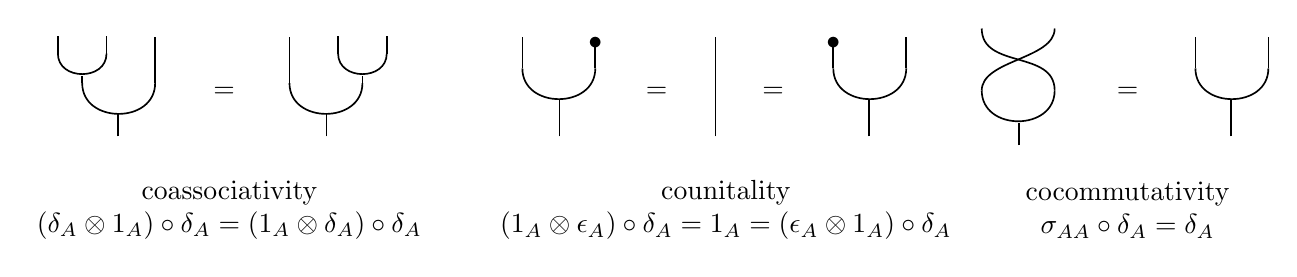
\begin{tikzpicture}[xscale = .65, yscale = .75, baseline=(current  bounding  box.center)]
\begin{pgfonlayer}{nodelayer}
		\node [style=none] (139) at (-1.625, 5.45) {};
		\node [style=none] (141) at (-1.625, 5.325) {};
		\node [style=none] (144) at (-2.1, 6.125) {};
		\node [style=none] (146) at (-2.1, 5.825) {};
		\node [style=none] (246) at (-0.925, 4.8) {};
		\node [style=none] (247) at (-0.925, 4.425) {};
		\node [style=none] (249) at (-0.2, 6.1) {};
		\node [style=none] (250) at (-0.2, 5.325) {};
		\node [style=none] (251) at (-1.15, 6.125) {};
		\node [style=none] (252) at (-1.15, 5.825) {};
		\node [style=none] (281) at (1.15, 5.175) {$=$};
		\node [style=none] (298) at (3.85, 5.45) {};
		\node [style=none] (299) at (3.85, 5.325) {};
		\node [style=none] (300) at (4.325, 6.125) {};
		\node [style=none] (301) at (4.325, 5.825) {};
		\node [style=none] (302) at (3.15, 4.8) {};
		\node [style=none] (303) at (3.15, 4.425) {};
		\node [style=none] (304) at (2.425, 6.1) {};
		\node [style=none] (305) at (2.425, 5.325) {};
		\node [style=none] (306) at (3.375, 6.125) {};
		\node [style=none] (307) at (3.375, 5.825) {};
		\node [style=none] (314) at (9.6, 5.175) {$=$};
		\node [style=none] (315) at (11.875, 5.175) {$=$};
		\node [style=none] (316) at (10.75, 6.1) {};
		\node [style=none] (317) at (10.75, 4.425) {};
		\node [style=none] (318) at (13.05, 6) {$\bullet$};
		\node [style=none] (319) at (13.05, 5.575) {};
		\node [style=none] (320) at (13.75, 5.05) {};
		\node [style=none] (321) at (13.75, 4.425) {};
		\node [style=none] (322) at (14.475, 6.1) {};
		\node [style=none] (323) at (14.475, 5.575) {};
		\node [style=none] (308) at (15.95, 6.25) {};
		\node [style=none] (309) at (17.375, 5.2) {};
		\node [style=none] (310) at (16.675, 4.65) {};
		\node [style=none] (311) at (16.675, 4.275) {};
		\node [style=none] (312) at (17.375, 6.25) {};
		\node [style=none] (313) at (15.95, 5.2) {};
		\node [style=none] (324) at (8.4, 6) {$\bullet$};
		\node [style=none] (325) at (8.4, 5.575) {};
		\node [style=none] (326) at (7.7, 5.05) {};
		\node [style=none] (327) at (7.7, 4.425) {};
		\node [style=none] (328) at (6.975, 6.1) {};
		\node [style=none] (329) at (6.975, 5.575) {};
		\node [style=none] (330) at (20.125, 6.1) {};
		\node [style=none] (331) at (20.125, 5.575) {};
		\node [style=none] (332) at (20.825, 5.05) {};
		\node [style=none] (333) at (20.825, 4.425) {};
		\node [style=none] (334) at (21.55, 6.1) {};
		\node [style=none] (335) at (21.55, 5.575) {};
		\node [style=none] (336) at (18.8, 5.175) {$=$};
		\node [style=none, label={[align=center]center: coassociativity\\$(\delta_A \otimes 1_A) \circ \delta_A =  (1_A \otimes \delta_A) \circ \delta_A$}] (337) at (1.25, 3.175) {};
		\node [style=none, label={[align=center]center:counitality\\$(1_A \otimes \epsilon_A) \circ \delta_A = 1_A = (\epsilon_A \otimes 1_A) \circ \delta_A$}] (338) at (10.95, 3.175) {};
		\node [style=none, label={[align=center]center:cocommutativity\\$\sigma_{AA} \circ \delta_A = \delta_A$}] (339) at (18.8, 3.175) {};
	\end{pgfonlayer}
	\begin{pgfonlayer}{edgelayer}
		\draw [style=wire] (141.center) to (139.center);
		\draw [style=wire] (146.center) to (144.center);
		\draw [style=wire] (247.center) to (246.center);
		\draw [style=wire] (250.center) to (249.center);
		\draw [style=wire] (252.center) to (251.center);
		\draw [style=wire, bend right=90, looseness=1.25] (141.center) to (250.center);
		\draw [style=wire, bend right=90, looseness=1.25] (146.center) to (252.center);
		\draw [style=wire] (299.center) to (298.center);
		\draw [style=wire] (301.center) to (300.center);
		\draw [style=wire] (303.center) to (302.center);
		\draw [style=wire] (305.center) to (304.center);
		\draw [style=wire] (307.center) to (306.center);
		\draw [style=wire, bend left=90, looseness=1.25] (299.center) to (305.center);
		\draw [style=wire, bend left=90, looseness=1.25] (301.center) to (307.center);
		\draw [style=wire] (311.center) to (310.center);
		\draw [style=wire] (317.center) to (316.center);
		\draw [style=wire] (319.center) to (318.center);
		\draw [style=wire] (321.center) to (320.center);
		\draw [style=wire] (323.center) to (322.center);
		\draw [style=wire, bend right=90, looseness=1.25] (319.center) to (323.center);
		\draw [style=wire, in=-90, out=90] (309.center) to (308.center);
		\draw [style=wire] (311.center) to (310.center);
		\draw [style=wire, in=-90, out=90, looseness=0.75] (313.center) to (312.center);
		\draw [style=wire, bend left=90, looseness=1.25] (309.center) to (313.center);
		\draw [style=wire] (325.center) to (324.center);
		\draw [style=wire] (327.center) to (326.center);
		\draw [style=wire] (329.center) to (328.center);
		\draw [style=wire, bend left=90, looseness=1.25] (325.center) to (329.center);
		\draw [style=wire] (331.center) to (330.center);
		\draw [style=wire] (333.center) to (332.center);
		\draw [style=wire] (335.center) to (334.center);
		\draw [style=wire, bend right=90, looseness=1.25] (331.center) to (335.center);
	\end{pgfonlayer}
\end{tikzpicture}
\end{equation}
Our convention is to draw a string diagram in the lower-left to upper-right direction. That is, composition is read from bottom to top and monoidal products from left to right. Therefore, above, the \memph{comultiplication} $\delta_A : A \fun A \otimes A$ is depicted as an upward fork
$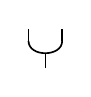
\begin{tikzpicture}[xscale = .3, yscale = .3, baseline={([yshift=5pt]current bounding box.south)}]
   \begin{pgfonlayer}{nodelayer}
		\node [style=none] (324) at (8.4, 6.1) {};
		\node [style=none] (325) at (8.4, 5.575) {};
		\node [style=none] (326) at (7.7, 5.05) {};
		\node [style=none] (327) at (7.7, 4.425) {};
		\node [style=none] (328) at (6.975, 6.1) {};
		\node [style=none] (329) at (6.975, 5.575) {};
	\end{pgfonlayer}
	\begin{pgfonlayer}{edgelayer}
		\draw [style=wire] (325.center) to (324.center);
		\draw [style=wire] (327.center) to (326.center);
		\draw [style=wire] (329.center) to (328.center);
		\draw [style=wire, bend left=90, looseness=1.25] (325.center) to (329.center);
	\end{pgfonlayer}
\end{tikzpicture}$
and the \memph{counit} $\epsilon_A : A \fun \moi$ an upward dead-end
$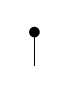
\begin{tikzpicture}[xscale = .3, yscale = .3, baseline={([yshift=5pt]current bounding box.south)}]
   \begin{pgfonlayer}{nodelayer}
		\node [style=none] (326) at (7.7, 5.8) {$\bullet$};
		\node [style=none] (327) at (7.7, 4.425) {};
	\end{pgfonlayer}
	\begin{pgfonlayer}{edgelayer}
		\draw [style=wire] (327.center) to (326.center);
	\end{pgfonlayer}
\end{tikzpicture}$.

Suppose that for each  object $A \in \cat C$ there are distinguished arrows $\delta_A : A \fun A \otimes A$, called the \memph{duplicate} on $A$, and $\epsilon_A : A \fun \moi$, called the \memph{discard} on $A$, that form a cocommutative monoidal comonoid as depicted in (\ref{mon:law}) (the qualifier ``distinguished'' is needed because there may be other such entities). Moreover, they respect the monoidal product:
\begin{equation}\label{fins:frob}
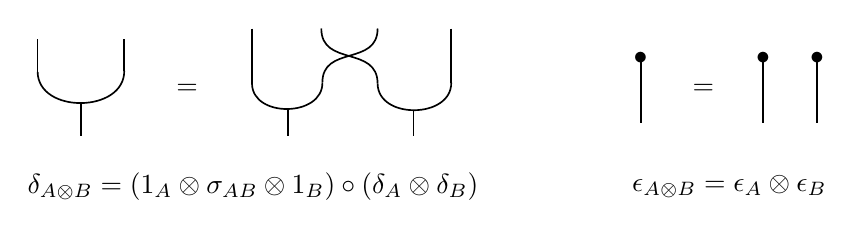
\begin{tikzpicture}[xscale = .55, yscale = .55, baseline=(current  bounding  box.center)]
\begin{pgfonlayer}{nodelayer}
		\node [style=none] (42) at (7.725, -0.75) {$=$};
		\node [style=none] (108) at (4.275, 0.4) {};
		\node [style=none] (110) at (6.275, 0.4) {};
		\node [style=none] (111) at (5.275, -1.825) {};
		\node [style=none] (112) at (4.275, -0.35) {};
		\node [style=none] (113) at (6.275, -0.325) {};
		\node [style=none] (114) at (5.275, -1.075) {};
		\node [style=none] (117) at (9.225, 0.65) {};
		\node [style=none] (118) at (12.125, 0.65) {};
		\node [style=none] (119) at (10.05, -1.825) {};
		\node [style=none] (120) at (9.225, -0.625) {};
		\node [style=none] (121) at (10.85, -0.6) {};
		\node [style=none] (122) at (10.05, -1.225) {};
		\node [style=none] (124) at (10.825, 0.65) {};
		\node [style=none] (125) at (13.825, 0.65) {};
		\node [style=none] (126) at (12.95, -1.825) {};
		\node [style=none] (127) at (12.125, -0.625) {};
		\node [style=none] (128) at (13.825, -0.6) {};
		\node [style=none] (129) at (12.95, -1.25) {};
		\node [style=none] (131) at (19.65, -0.75) {$=$};
		\node [style=none] (134) at (18.2, -1.525) {};
		\node [style=none] (137) at (18.2, -0.05) {$\bullet$};
		\node [style=none] (138) at (20.25, -3) {$\epsilon_{A \otimes B} = \epsilon_{A} \otimes \epsilon_{B}$};
		\node [style=none] (145) at (21.025, -1.525) {};
		\node [style=none] (146) at (21.025, -0.05) {$\bullet$};
		\node [style=none] (148) at (22.275, -1.525) {};
		\node [style=none] (149) at (22.275, -0.05) {$\bullet$};
		\node [style=none] (151) at (9.25, -3) {$\delta_{A \otimes B} = (1_A \otimes \sigma_{AB} \otimes 1_B) \circ (\delta_{A} \otimes \delta_B)$};
	\end{pgfonlayer}
	\begin{pgfonlayer}{edgelayer}
		\draw [style=wire, bend right=90, looseness=1.25] (112.center) to (113.center);
		\draw [style=wire] (108.center) to (112.center);
		\draw [style=wire] (110.center) to (113.center);
		\draw [style=wire] (111.center) to (114.center);
		\draw [style=wire, bend right=90, looseness=1.25] (120.center) to (121.center);
		\draw [style=wire] (117.center) to (120.center);
		\draw [style=wire, in=90, out=-90, looseness=1.25] (118.center) to (121.center);
		\draw [style=wire] (119.center) to (122.center);
		\draw [style=wire, bend right=90, looseness=1.25] (127.center) to (128.center);
		\draw [style=wire, in=90, out=-90, looseness=1.25] (124.center) to (127.center);
		\draw [style=wire] (125.center) to (128.center);
		\draw [style=wire] (126.center) to (129.center);
		\draw [style=wire] (134.center) to (137.center);
		\draw [style=wire] (145.center) to (146.center);
		\draw [style=wire] (148.center) to (149.center);
	\end{pgfonlayer}
\end{tikzpicture}
\end{equation}
Here and below, the associators and unitors of $\cat C$ are suppressed, in the diagrams as well as in the accompanying equations. For instance, the counitality law in (\ref{mon:law}) is read after identifying $A \otimes \moi$ and $\moi \otimes A$ with $A$, and the right-hand side of the second equation in (\ref{fins:frob}) is followed by the canonical isomorphism $\moi \otimes \moi \cong \moi$.

Following \cite{fritz2020synthetic}, we call $\cat C$ a \memph{Markov category} if the  discards are natural, that is, they are the component morphisms of the natural transformation between the identity functor $1_{\cat C}$ and the endofunctor that sends everything to $\moi$:
\begin{equation}\label{discar:nat}
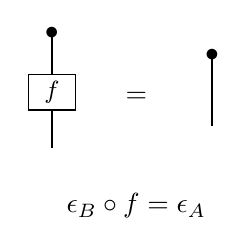
\begin{tikzpicture}[xscale = .55, yscale = .55, baseline=(current  bounding  box.center)]
	\begin{pgfonlayer}{nodelayer}
		\node [style=none] (200) at (19.4, 1.75) {$=$};
		\node [style=none] (202) at (17.45, 1.525) {};
		\node [style=none] (205) at (17.45, 0.6) {};
		\node [style=small box] (207) at (17.45, 1.875) {$f$};
		\node [style=none] (208) at (17.45, 3.225) {$\bullet$};
		\node [style=none] (209) at (17.45, 2.3) {};
		\node [style=none] (210) at (21.15, 2.725) {$\bullet$};
		\node [style=none] (211) at (21.15, 1.1) {};
		\node [style=none] (212) at (19.4, -0.75) {$\epsilon_B \circ f = \epsilon_A$};
	\end{pgfonlayer}
	\begin{pgfonlayer}{edgelayer}
		\draw [style=wire] (202.center) to (205.center);
		\draw [style=wire] (208.center) to (209.center);
		\draw [style=wire] (210.center) to (211.center);
	\end{pgfonlayer}
\end{tikzpicture}
\end{equation}
However, it is unreasonable to also require duplicates to be natural, see the opening discussion in \cite[\S~10]{fritz2020synthetic}.

We may forego this discussion on the naturality of discards if the monoidal unit $\moi$ is actually terminal, since in that case the desired property would hold automatically; conversely, the naturality of discards, together with the other conditions stipulated above, implies that  $\moi$ is terminal, and hence $\epsilon_\moi  = 1_\moi$. Also note that $\delta_\moi = 1_\moi$  in any strict Markov category. See \cite[Remark~2.3]{fritz2020synthetic}.

Accordingly, a \memph{Markov functor} is a strong symmetric monoidal functor  $F : \cat C \fun \cat D$ between two Markov categories that preserves the distinguished  comonoids by way of matching duplicates and discards, that is, for all objects $A \in \cat C$, the diagrams
\begin{equation*}
  \bfig
      \Atriangle(0,0)/->`->`->/<400,400>[FA`FA \otimes FA`F(A \otimes A); \delta_{FA}`F\delta_A`\cong]
      \Atriangle(1500,0)/->`->`->/<250,400>[FA`\moi`F \moi; \epsilon_{FA}`F\epsilon_A`\cong]
  \efig
\end{equation*}
commute, where  the horizontal arrows are the structure isomorphisms in question; see \cite[Definition~10.14]{fritz2020synthetic}. Of course the discards are matched automatically, since $\moi$ is terminal. Denote by \cat{MarCat} the category of Markov categories and Markov functors. In this paper, for simplicity,  \cat{MarCat} is only implicitly treated as a $2$-category when we occasionally speak of \memph{comonoid equivalence}, that is, equivalence in \cat{MarCat}.

To formulate the notion of a free Markov category, as in \cite{selinger2010survey}, we first need to fix a suitable class of signatures (called ``tensor schemes'' in \cite{joyal1991geometry}), as follows.

A \memph{graph monoid} is a directed graph $G = (V(G), A(G), s, t)$ whose set of vertices comes with the additional structure of a monoid. A \memph{graph monoid homomorphism} is a graph homomorphism that is also a homomorphism between the monoids in question.

For any set $S$, let $W(S)$ denote the free monoid of words over (the alphabet) $S$. It is a graph monoid, with the trivial directed graph structure (no arrows). More generally, a \memph{free graph monoid} is a triple $(G, S, g)$, where $G$ is a graph monoid and $g : S \fun V(G)$ is an injection, such that the monoid $V(G)$ is isomorphic to the free monoid $W(S)$ over $g$. We usually just say $G$ is a free graph monoid and leave $S$, $g$ implicit in notation when they are not needed in the discussion. Also it is harmless to treat $S$ as if it is a subset of $V(G)$.

A \memph{free $\DD$-graph monoid} is a free graph monoid $(G, S, g)$ such that, for each $a \in S$, there are distinguished arrows $a \fun aa$, called the \memph{duplicate} on $a$, and $a \fun \0$, called the \memph{discard} on $a$.



A Markov category is \memph{strict} if its underlying monoidal category is, and a Markov functor is \memph{strict} if its structure isomorphisms are identities. If $\cat D$ is a strict Markov category then $\cat D_0$ is a monoid under $\otimes$, and hence the underlying graph of $\cat D$ is a graph monoid. A graph monoid homomorphism $f : G \fun \cat D$ from a free $\DD$-graph monoid $G$ \memph{matches duplicates and discards} if it sends the duplicate and the discard on each $a \in S$ to $\delta_{f(a)}$ and $\epsilon_{f(a)}$, respectively.

A strict Markov category $\cat C$ is \memph{free} over a free $\DD$-graph monoid $G$ if there is a graph monoid homomorphism $i : G \fun \cat C$ matching duplicates and discards such that, for any strict Markov category $\cat D$, any graph monoid homomorphism $f : G \fun  \cat D$ matching duplicates and discards factors uniquely through $i$, that is, there is exactly one strict Markov functor $F : \cat C \fun \cat D$ such that $f = F \circ i$. The objects and morphisms in $i(G)$ are referred to as \memph{generators}.

The restriction to strict Markov categories is harmless, since every Markov category is comonoid equivalent to a strict one \cite[Theorem~10.17]{fritz2020synthetic}. On the other hand, the strictness of $F$ cannot simply be replaced by uniqueness up to a unique monoidal natural isomorphism. For instance, let $S = \{a\}$, with the duplicate and the discard on $a$ the only arrows of $G$, and let $f(a)$ be a two-element set in a strict Markov category that is comonoid equivalent to the category of finite sets with its cartesian product. The transposition of $f(a)$ commutes with duplicating and discarding, and hence its tensor powers form a monoidal natural automorphism of $F$ other than the identity. For a $2$-categorical universal property with arbitrary targets, which keeps track of such comparison isomorphisms, see \cite[Theorem~6.6]{FriLiang2022}; the strict version is \cite[Corollary~6.7]{FriLiang2022}.


Since Markov categories are symmetric monoidal categories, the same graphical language can be used, but  with the additional syntax depicted in (\ref{mon:law}), (\ref{fins:frob}), and (\ref{discar:nat}). This does not give the free  Markov category over a free $\DD$-graph monoid, though, at least not for string diagrams up to isomorphisms. We need a coarser equivalence relation to accommodate the equations in  (\ref{mon:law}), (\ref{fins:frob}), and (\ref{discar:nat}).

\begin{rem}
The surgery method described in this paper works  rather well in some applications where free Markov categories play an essential role, see \cite{yinzhang2021}. For other monoidal categories with more complex conditions, it is not that the method does not work, it is just that the equivalence relation so constructed may be hard to parse visually, and consequently working with a graphical language does not seem to offer advantages over a symbolic one, which in a sense defeats the purpose of graphical languages.

For the construction of free Markov categories, there is a more sophisticated combinatorial approach, see \cite{FriLiang2022}.
\end{rem}


\section{Preliminaries on Joyal-Street style diagrams}

The discussion below assumes familiarity with the first two chapters of  \cite{joyal1991geometry}. We begin by recalling some definitions therein.

A \memph{generalized topological graph} $\Gamma = (\Gamma, \Gamma_0)$ consists of a Hausdorff space $\Gamma$ and a finite subset $\Gamma_0 \sub  \Gamma$ such that the complement $\Gamma \mi  \Gamma_0$ is a one-dimensional manifold without boundary and with finitely many connected components. We require that each of the connected components of $\Gamma \mi  \Gamma_0$ be homeomorphic to the open unit interval $(0, 1) \sub \R$, that is, there are no circles.

An element of $\Gamma_0$ is called a \memph{node}. A connected component of $\Gamma \mi \Gamma_0$ is called an \memph{edge}. The set of edges of $\Gamma$ is denoted by $\Gamma_1$. The  compactification $\hat e$ of an edge $e$, obtained by adjoining two endpoints, is homeomorphic to the closed unit interval $[0, 1] \sub \R$. An edge $e$ is called \memph{pinned} if the inclusion $e \sub \Gamma$ can be extended to a continuous map $\hat e  \fun \Gamma$, and \memph{half-loose} if it can only be extended to $\hat e$ minus one endpoint,  and \memph{loose} if neither of the previous two cases holds.

Let $\overline \Gamma$ be the compactification of $\Gamma$ obtained by adjoining one endpoint to each half-loose edge and two endpoints to each loose edge (this is not the one-point compactification, which would identify the two ends of a loose edge), and write $\partial \Gamma$ for the set $\overline \Gamma \mi \Gamma$. The points in $\partial \Gamma$ are referred to as the \memph{outer nodes} of $\Gamma$ (nodes in $\Gamma_0$ are also called \memph{inner nodes} for clarity). Note that $\partial \Gamma$ and $\Gamma_0$ together form the boundary of $\Gamma$. The inclusion $e \sub \Gamma$ of every edge $e$ now extends to a continuous map $\hat e \fun \overline \Gamma$.

An \memph{orientation} of an edge $e$ is just a total ordering on the pair of endpoints of $\hat e$, where the \memph{source} $e(0)$ is the image of the first element under the induced map $\hat e \fun  \overline \Gamma$ and the
\memph{target} $e(1)$ that of the last element. We say that $\Gamma$ is \memph{progressive} if it carries a choice of orientation for
each of its edges such that there is no directed circuit, that is, no sequence of edges $e_1, \ldots, e_n$, $n \geq 1$, with $e_i(1) = e_{i+1}(0)$ for $i < n$ and $e_n(1) = e_1(0)$ (circuits that are not directed are allowed; for instance, two edges may have the same source and the same target). In that case, the \memph{input} $\inn(x)$ of a node $x \in \Gamma_0$ is the set of the oriented edges with target $x$ and the \memph{output} $\out(x)$ the set of those with source $x$. An inner node $x \in \Gamma_0$ is \memph{initial} if $\inn(x) = \0$ and \memph{terminal} if $\out(x) = \0$. If, in addition, $\Gamma$ is equipped with a choice of total orderings on $\inn(x)$ and $\out(x)$ for each $x \in \Gamma_0$ then it is  \memph{polarized}. We shall only consider polarized graphs and hence may omit the qualifier for brevity.

The \memph{domain} $\dom(\Gamma)$ of $\Gamma$ consists of the edges whose sources are outer nodes and the \memph{codomain} $\cod(\Gamma)$ those whose targets are outer nodes. The edges in $\dom(\Gamma)$, $\cod(\Gamma)$ are often identified with the corresponding outer nodes for convenience. We say that $\Gamma$ is \memph{anchored} if both $\dom(\Gamma)$ and $\cod (\Gamma)$ are equipped with a total ordering.


\begin{defn}
Let $\cat C$ be a symmetric strict monoidal category. A \memph{valuation} $v : \Gamma \fun \cat C$ is a pair of functions
\[
v_1 : \Gamma_0 \fun \cat C_1, \quad v_0 : \Gamma_1 \fun \cat C_0
\]
such that, for every node $x \in  \Gamma_0$ with $\inn(x) = (a_1, \ldots, a_n)$ and $\out(x) = (b_1, \ldots, b_m)$, $v_1(x)$ is of the form $\bigotimes_i v_0(a_i) \fun \bigotimes_i v_0(b_i)$; here if $n = 0$ or $m = 0$ then the monoidal product in question is just the monoidal unit $\moi$ of $\cat C$. The pair $(\Gamma, v)$ is called a  \memph{diagram}  in $\cat C$, and is denoted simply by $\Gamma$ when the context is clear. If $\Gamma$ is anchored then the  domain $\dom(\Gamma, v)$ of $(\Gamma, v)$ is the object $\bigotimes_{e_i \in \dom(\Gamma)} v_0(e_i)$, where the monoidal product is taken with respect to the ordering on $\dom(\Gamma)$, similarly for the codomain $\cod(\Gamma, v)$ of $(\Gamma, v)$.

An \memph{isomorphism of  diagrams} $\Gamma \fun \Omega$ is an isomorphism of the  graphs  that  is compatible with the valuations in the obvious way. If the graphs are anchored then the isomorphism is required to preserve the anchoring too.

A diagram in a free  graph monoid $(G, S, g)$ is formulated in the same way,  with the valuation $v : \Gamma \fun (G, S, g)$ mapping the edges and nodes into the alphabet $S$ and the set $A(G)$ of arrows, respectively; that is, for $x$ as above, $v_1(x)$ is an arrow of $G$ from the word $v_0(a_1) \cdots v_0(a_n)$ to the word $v_0(b_1) \cdots v_0(b_m)$ (the empty word if $n = 0$, respectively $m = 0$), and the domain and the codomain of an anchored diagram are the corresponding words over $S$.
\end{defn}


\begin{rem}\label{free:sys:mo:string}
Isomorphisms of graphs are homeomorphisms of one-dimensional topological spaces and, insofar as diagrams in  symmetric monoidal categories are concerned, they can be equivalently replaced by ambient isotopies of graphs embedded in $\R^4$, but not in lower dimensions. The reason is simply that, in the graphical language of symmetric monoidal categories,  we represent a symmetry as a braid, which is then forced by the axioms to coincide with its inverse, and indeed a braid in $\R^4$ is determined, up to isotopy, by the permutation of the endpoints that it induces. For instance, the crossing in the third diagram of (\ref{mon:law}) is  a projection in $\R^2$ of the symmetry braid in $\R^4$, and there is no need to depict, between the two strands, which one lies over which one, precisely because all the cases represent the same braid, that is, the one that exchanges the two endpoints. Thus, the intersection point therein is not a node of the graph, it is merely the (intentional) overlap of the shadows in $\R^2$ of the two edges, which do not intersect in $\R^4$ at all.
\end{rem}

Let $(G, S, g)$ be a free graph monoid. Recall from \cite[Chapter~2, \S~2]{joyal1991geometry} how the anchored diagrams in $G$ are assembled into a symmetric strict monoidal category $\cat F_s(G)$. The objects are the words over $S$. The arrows are the isomorphism classes $[\Gamma, v]$ of anchored diagrams $(\Gamma, v)$ in $G$, from the word $\dom(\Gamma, v)$ to the word $\cod(\Gamma, v)$. If $\cod(\Gamma, v) = \dom(\Omega, w)$ then $[\Omega, w] \circ [\Gamma, v]$ is represented by the diagram obtained from the disjoint union of $\Gamma$ and $\Omega$ by identifying the outer nodes in $\cod(\Gamma)$ with those in $\dom(\Omega)$ in the given order and then removing them, so that each pair of edges thus matched becomes a single edge. The monoidal product $[\Gamma, v] \otimes [\Omega, w]$ is represented by the disjoint union of $\Gamma$ and $\Omega$, with the orderings of the domains, and of the codomains, concatenated. The identities and the symmetries are represented by diagrams without inner nodes, where the orderings of the domain and the codomain differ by the permutation in question.

\begin{thm}[{\cite[Theorem~2.3]{joyal1991geometry}}]\label{free:sym}
The isomorphism classes of anchored diagrams $(\Gamma, v)$ in the free  graph monoid $G$, denoted by $[\Gamma, v]$, form the free symmetric monoidal category $\cat F_s(G)$ over $G$.
\end{thm}

Here freeness is understood as in the Introduction, without the duplicates and the discards: every graph monoid homomorphism from $G$ into a symmetric strict monoidal category factors through the obvious graph monoid homomorphism $G \fun \cat F_s(G)$ by exactly one strict symmetric monoidal functor; see the proof of \cite[Theorem~2.3]{joyal1991geometry} and the remark after the proof of \cite[Theorem~1.2]{joyal1991geometry}.

From here on we assume that $\Gamma$ is anchored.

A \memph{directed path} $p$ in $\Gamma$ is a sequence of edges $e_1, \ldots, e_n$, $n \geq 1$, with $e_i(1) = e_{i+1}(0)$ for $i < n$; we write $p(0) = e_1(0)$ and $p(1) = e_n(1)$, which may be inner or outer nodes. Recall  that  $\Gamma_0$  may be ordered as follows: $x < y$ if and only if there is a directed path $p$ in $\Gamma$ from $p(0) = x$ to $p(1) = y$. This is a strict partial ordering since there are no directed circuits, and we write $x \leq y$ if $x < y$ or $x = y$; the thus formed  partially ordered set is denoted by $\dot\Gamma$.

An initial segment of $\dot \Gamma$ is referred to as a \memph{level} of $\Gamma$, with $\0$ the smallest one and $\dot \Gamma$ the largest one.

An edge $e$ is said to be \memph{cut} by a level $L$ when $e(0) \in L \cup \dom(\Gamma)$ and $e(1) \in (\dot \Gamma \mi L) \cup \cod(\Gamma)$. Here the edges in $\dom(\Gamma)$, $\cod(\Gamma)$ are identified with the corresponding outer nodes, as before; so the first condition holds if $e(0)$ is an outer node, similarly for the second one, and a loose edge of $\Gamma$ is cut by every level.

A \memph{subgraph} $\Gamma'$ of $\Gamma$ is given by a subset $\Gamma'_0 \sub \Gamma_0$ and a subset $\Gamma'_1 \sub \Gamma_1$; as a space it is the union of $\Gamma'_0$ and the edges in $\Gamma'_1$, and $(\Gamma', \Gamma'_0)$ is again a graph. Thus if an end of an edge $e \in \Gamma'_1$ is attached in $\Gamma$ to a node outside $\Gamma'_0$ then, in $\Gamma'$, it is attached to an outer node of its own; in particular, $e$ is pinned in $\Gamma'$ if and only if both $e(0)$ and $e(1)$ belong to $\Gamma'_0$, and loose in $\Gamma'$ if and only if neither does.

Let $\cut(L)$ denote the set of edges cut by $L$; we have $\cut(\0) = \dom(\Gamma)$ and $\cut(\dot \Gamma)  = \cod(\Gamma)$. For a pair of levels $L \sub M$, the \memph{layer} $\Gamma[L, M]$ in $\Gamma$ is the subgraph of $\Gamma$ such that
\begin{itemize}
  \item its inner nodes are those in $M \mi L$,
  \item its pinned edges are those $e \in \Gamma_1$ with $e(0), e(1) \in M \mi L$,
  \item its loose and half-loose edges are those in $\cut(L) \cup \cut(M)$.
\end{itemize}
So $\cut(L) = \dom(\Gamma[L, M])$ and $\cut(M) = \cod(\Gamma[L, M])$, and the loose edges are exactly those in $\cut(L) \cap \cut(M)$, in particular, $\dom(\Gamma) = \dom(\Gamma[\0, L])$ and $\cod(\Gamma) = \cod(\Gamma[L, \dot \Gamma])$.



Any subgraph $\Gamma' \sub \Gamma$ inherits the orientations of the edges and the total orderings of $\inn_{\Gamma'}(x) \sub \inn_{\Gamma}(x)$, $\out_{\Gamma'}(x) \sub \out_{\Gamma}(x)$ for each $x \in \Gamma'_0$, and hence is  polarized. On the other hand, there is not a natural way to order $\dom(\Gamma') \mi \dom(\Gamma)$ or $\cod(\Gamma') \mi \cod(\Gamma)$, so $\Gamma'$ is not naturally anchored unless these two sets are empty.

\begin{rem}\label{order:raley:com}
Since a layer $\Gamma[L, M]$ is not naturally anchored, it cannot be used as is to produce a morphism in  $\cat F_s(G)$. If we choose total orderings on the domain and codomain then of course $\Gamma[L, M]$ may be turned into an anchored graph, although different choices in general bring about nonisomorphic results. In some situations, what  orderings we choose is immaterial,  as long as they are compatible. For instance, if $\Gamma_1$, $\Gamma_2$, and $\Gamma_3$ are only equipped with partial orderings on the domains and codomains then by writing
\[
[\Gamma, v] = [\Gamma_3, v_3] \circ [\Gamma_2, v_2] \circ [\Gamma_1, v_1]
\]
we mean that the partial orderings may be extended to compatible total orderings so as to make the equality hold. In particular, this shall be what is meant when we write
\[
[\Gamma, v] = [\Gamma[M, \dot \Gamma], v_3] \circ [\Gamma[L, M], v_2] \circ [\Gamma[\0, L], v_1],
\]
where $v_1$, $v_2$, and $v_3$ are the induced valuations.
\end{rem}

\section{Surgeries on diagrams}

We continue to work with an anchored graph $\Gamma$.

\begin{defn}\label{def:full}
We say that a subgraph $\Gamma' \sub \Gamma$ is \memph{normal} if
\begin{itemize}
  \item no directed path in $\Gamma$ contains two distinct edges in $\Gamma'$ if one of them is loose in $\Gamma'$,
  \item the degree of every $x \in \Gamma'_0$ in $\Gamma'$ is the same as in $\Gamma$, in other words, all the edges at $x$ in $\Gamma$ are included in $\Gamma'$,
  \item every directed path  $p$ in $\Gamma$ with $p(0), p(1) \in \Gamma'_0$ belongs to  $\Gamma'$.
\end{itemize}
\end{defn}

For a subgraph $\Gamma' \sub \Gamma$, let $\Gamma'^{\flat}$ denote the subgraph obtained from $\Gamma'$ by deleting its loose edges.

Observe that if two subgraphs $\Gamma'$, $\Gamma''$ have the same set of nodes and both satisfy the second  condition above then $\Gamma'^{\flat}$, $\Gamma''^{\flat}$ must be equal. Also, in a normal subgraph $\Gamma'$ of $\Gamma$, if $x \in  \Gamma'_0$ is initial in $\Gamma'$ then it is initial in $\Gamma$, similarly if it is terminal.


\begin{lem}\label{full:lay}
A subgraph $\Gamma' \sub \Gamma$ is normal if and only if there is a layer $\Gamma[L, M]$ in $\Gamma$ such that $\Gamma' \sub \Gamma[L, M]$ and $\Gamma[L, M]^\flat = \Gamma'^{\flat}$.
\end{lem}
\begin{proof}
For the ``if'' direction, it is enough to show that $\Gamma[L, M]$ is normal, because deleting loose edges from a normal subgraph leaves it normal (the edges required by the second and the third conditions in Definition~\ref{def:full} have an endpoint among its nodes, and hence are not loose in it). First, let $p$ be a directed path in $\Gamma$. Suppose for contradiction that $p$ contains two distinct edges $e$, $e'$ in $\Gamma[L, M]$, where $e$ is loose in $\Gamma[L, M]$. We have, in $\dot \Gamma$, either $e(1) \leq e'(0)$ or $e'(1) \leq e(0)$. For the first case, since $e$ is cut by $M$, we have $e(1) \in \dot \Gamma \mi M$ and hence $e'(0) \in \dot \Gamma \mi M$, which entails that  $e'$ cannot be in $\Gamma[L, M]$, contradiction. Similarly, for the second case, since $e$ is cut by $L$ as well, we have $e(0) \in L$ and hence $e'(1) \in  L$, so  $e'$ cannot be in $\Gamma[L, M]$, contradiction again. Next, if $p(0), p(1) \in \Gamma[L, M]_0 = M \mi L$ then clearly $p$ belongs to $\Gamma[L, M]$. Lastly, for any $x \in \Gamma[L, M]_0$, if $e \in \inn_\Gamma(x)$ is cut by $L$ then it belongs to $\Gamma[L, M]$ by definition, otherwise $e(0) \in M \mi L$ and hence $e$ still belongs to $\Gamma[L, M]$ by definition, similarly for $e \in \out_\Gamma(x)$. So $\Gamma[L, M]$ is normal.

For the ``only if'' direction, let $\Gamma' \sub \Gamma$ be normal. Let $L$ be the set of the nodes $x \in \dot \Gamma$ such that either $x \notin \Gamma'_0$ and $x < y$ for some $y \in \Gamma'_0$ or $x \leq  e(0) \in \dot \Gamma$ for some loose edge $e$ in $\Gamma'$. If the first case holds and $z < x$ then $z \notin \Gamma'_0$, for otherwise $z < x < y$ and hence $x \in \Gamma'_0$ too by the third condition in Definition~\ref{def:full}, contradiction. So $L$ is a level. Actually, if $x \leq  e(0) \in \dot \Gamma$ for some loose edge $e$ in $\Gamma'$  then $x \notin  \Gamma'_0$, for otherwise $x < e(0)$ (note that $e(0) \notin \Gamma'_0$ since $e$ is loose in $\Gamma'$) and there would be a directed path in $\Gamma$ that contains $e$ and an edge $e'$ at $x$, and since $e' \in \Gamma'$ by the second condition in Definition~\ref{def:full}, this contradicts the first condition therein. So  $L \cap \Gamma'_0 = \0$. Now, let $M$ be the set of the nodes $x \in \dot \Gamma$ such that $x \leq y$ for some $y \in \Gamma'_0$ or $x \leq e(0) \in \dot \Gamma$ for some loose edge $e$ in $\Gamma'$.  Clearly $M$ is a level and contains $L$. We have $M \mi L = \Gamma'_0$.

Since $\Gamma[L, M]^{\flat}$ is normal too, we have $\Gamma[L, M]^{\flat} = \Gamma'^{\flat}$. For any loose edge $e$ in $\Gamma'$, if $e(1) \in M$ then there would be a directed path in $\Gamma$ that contains two distinct edges in $\Gamma'$, one of which is $e$,  contradicting the first condition in Definition~\ref{def:full}, so  $e$ is cut by both $L$ and $M$, in other words, $e$ is a loose edge in $\Gamma[L, M]$. So $\Gamma' \sub \Gamma[L, M]$.
\end{proof}

Denote by $\Gamma'^{\sharp}$ the layer $\Gamma[L, M]$ constructed from $\Gamma'$ in the latter half of the proof above.

So normal subgraphs are almost the same as layers. The point, of course, is that they are more intuitive to work with.

Suppose that $\Gamma' \sub \Gamma$ is a normal subgraph. Let $\phi : \Omega \fun \Gamma'$ be an isomorphism of  graphs. Let $\Lambda$ be a  graph and
\[
\alpha : \dom(\Lambda) \fun \dom(\Omega), \quad \beta: \cod(\Lambda) \fun \cod(\Omega)
\]
bijections. We can graft $\Lambda$ onto $\Gamma$ by identifying the edges in $\dom(\Lambda)$, $\cod(\Lambda)$ with the corresponding edges in $\Gamma'$ --- for this to work, the loose edges in $\Gamma'$ need to be duplicated, with one copy each in $\dom(\Gamma')$ and $\cod(\Gamma')$ ---  and then cut out the rest of $\Gamma'$ from $\Gamma$. We call this operation the \memph{$(\Omega / \Lambda, \phi, \alpha, \beta)$-surgery} on $\Gamma$ and write $\Gamma^\Omega_\Lambda(\phi, \alpha, \beta)$ for the resulting graph, where $\phi$, $\alpha$, and $\beta$ shall be dropped from the notation when the context is clear; the triple $(\Omega / \Lambda, \alpha, \beta)$ is referred to as the \memph{template} of the surgery.

More precisely, write $\Gamma'^{\sharp} = \Gamma[L, M]$ and let $R$ be the set of the loose edges of $\Gamma[L, M]$ that are not in $\Gamma'$, so that $\cut(L) = \dom(\Gamma') \uplus R$ and $\cut(M) = \cod(\Gamma') \uplus R$ by Lemma~\ref{full:lay}. Let $\Lambda^{\sharp} = \Lambda \uplus R$, where the edges in $R$ are loose. Then $\Gamma^\Omega_\Lambda$ is obtained from the disjoint union of $\Gamma[\0, L]$, $\Lambda^{\sharp}$, and $\Gamma[M, \dot \Gamma]$ by gluing $\cod(\Gamma[\0, L]) = \cut(L)$ to $\dom(\Lambda^{\sharp})$ and $\cod(\Lambda^{\sharp})$ to $\dom(\Gamma[M, \dot \Gamma]) = \cut(M)$, in the same way as in the composition of $\cat F_s(G)$, along the bijections given by $\phi \circ \alpha$, $\phi \circ \beta$, and the identity on $R$. A directed path in $\Gamma^\Omega_\Lambda$ never passes from one of the three pieces back into an earlier one, so there are no directed circuits, and the orderings of $\inn(x)$, $\out(x)$ are inherited from the pieces; thus $\Gamma^\Omega_\Lambda$ is again a graph in our sense. This is where the normality of $\Gamma'$ is used.

Clearly there are induced bijections
\[
\alpha^\sharp : \dom(\Gamma^\Omega_\Lambda) \fun \dom(\Gamma), \quad \beta^\sharp:  \cod(\Gamma^\Omega_\Lambda) \fun \cod(\Gamma)
\]
and hence $\Gamma^\Omega_\Lambda$ is indeed naturally anchored; in particular, if there is an isomorphism $\Lambda \fun \Omega$ of polarized graphs that induces $\alpha$ and $\beta$ then $\Gamma^\Omega_\Lambda$ is isomorphic to $\Gamma$ (as anchored polarized graphs). If the template is empty, that is, if $\Lambda = \Omega = \0$, then $\Gamma^\Omega_\Lambda = \Gamma$.


Let $G$ be a free graph monoid. Let $v : \Gamma \fun G$, $w : \Lambda \fun G$,  and $u : \Omega \fun G$ be valuations. Let $\phi : (\Omega, u) \fun (\Gamma', v')$ be an isomorphism of  diagrams, where  $v'$ is the restriction of $v$ to $\Gamma'$. Suppose that $u$, $w$ are compatible with respect to $\alpha$ and $\beta$, that is, $w(e) = (u \circ \alpha)(e)$ for $e \in \dom(\Lambda)$,  and similarly for $e \in \cod(\Lambda)$. Since $\Gamma' \sub \Gamma$ is normal, there is an induced valuation $v_w : \Gamma^\Omega_\Lambda \fun G$ fusing $v$, $w$ together such that $v_w(e) = (v \circ \alpha^\sharp)( e)$ for $e \in \dom(\Gamma^\Omega_\Lambda)$, and similarly for  $e \in \cod(\Gamma^\Omega_\Lambda)$. So \[
\dom(\Gamma^\Omega_\Lambda, v_w) = \dom(\Gamma, v) \dand \cod(\Gamma^\Omega_\Lambda, v_w) = \cod(\Gamma, v).
\]
The transition from the diagram $(\Gamma, v)$ to the diagram $(\Gamma^\Omega_\Lambda, v_w)$ is called the \memph{$((\Omega, u) / (\Lambda, w), \phi, \alpha, \beta)$-surgery} on $(\Gamma, v)$ with the \memph{template} $((\Omega, u) / (\Lambda, w), \alpha, \beta)$; again,  we usually only show $\Omega / \Lambda$ in notation.

Observe that a surgery can be reversed (by another surgery) in the sense that the resulting diagram is isomorphic to the one we started with.

\begin{lem}\label{sur:decom}
Let $((\Omega, u) / (\Lambda, w), \alpha, \beta)$ be a template. An anchored diagram $(\Xi, t)$ is isomorphic to the result of a surgery on $(\Gamma, v)$ with this template if and only if there are
\begin{itemize}
  \item a normal subgraph $\Gamma' \sub \Gamma$ and an isomorphism of diagrams $\phi : (\Omega, u) \fun (\Gamma', v')$,
  \item total orderings that anchor $\Gamma'^{\sharp}$ and $\Lambda^{\sharp}$ such that the bijections $\dom(\Lambda^{\sharp}) \fun \dom(\Gamma'^{\sharp})$ and $\cod(\Lambda^{\sharp}) \fun \cod(\Gamma'^{\sharp})$ given by $\phi \circ \alpha$, $\phi \circ \beta$, and the identity on $\Gamma'^{\sharp} \mi \Gamma'$ are order-preserving,
  \item morphisms $g$, $h$ in $\cat F_s(G)$
\end{itemize}
such that
\[
h \circ [\Gamma'^{\sharp}, v'^{\sharp}] \circ g = [\Gamma, v] \dand h \circ [\Lambda^{\sharp}, w^{\sharp}] \circ g = [\Xi, t],
\]
where $v'^{\sharp}$ is the restriction of $v$ to $\Gamma'^{\sharp}$, $\Lambda^{\sharp} = \Lambda \uplus (\Gamma'^{\sharp} \mi \Gamma')$,  and  $w^{\sharp} = w \uplus (v \rest (\Gamma'^{\sharp} \mi \Gamma'))$.
\end{lem}
\begin{proof}
For the ``only if'' direction, let $\Gamma' \sub \Gamma$ be the normal subgraph and $\phi$ the isomorphism in question, write $\Gamma'^{\sharp} = \Gamma[L, M]$, and choose total orderings as in the second item. Then, by the construction of $\Gamma^\Omega_\Lambda$,
\begin{gather*}
[\Gamma, v] = [\Gamma[M, \dot \Gamma], v_M] \circ [\Gamma'^{\sharp}, v'^{\sharp}] \circ [\Gamma[\0, L], v_L],\\
[\Xi, t] = [\Gamma[M, \dot \Gamma], v_M] \circ [\Lambda^{\sharp}, w^{\sharp}] \circ [\Gamma[\0, L], v_L].
\end{gather*}
where $v_M$, $v_L$ are the induced valuations; here we have used the convention outlined in Remark~\ref{order:raley:com}.

For the ``if'' direction, represent $g$, $[\Gamma'^{\sharp}, v'^{\sharp}]$, and $h$ by diagrams. The first equality gives an isomorphism from the diagram glued from the three of them onto $(\Gamma, v)$, under which the middle one corresponds to a layer of $\Gamma$ and $\Gamma'$ to a subgraph $\Gamma''$ of $\Gamma$, which is normal by Lemma~\ref{full:lay} (it need not be $\Gamma'$ itself). By the second equality, $(\Xi, t)$ is isomorphic to the result of the corresponding surgery on $\Gamma''$, because the construction of $\Gamma^\Omega_\Lambda$ does not depend on the choice of a layer $\Gamma[L, M]$ with $\Gamma' \sub \Gamma[L, M]$ and $\Gamma[L, M]^\flat = \Gamma'^{\flat}$: the nodes of $\Gamma^\Omega_\Lambda$, its edges, and their incidences are determined by $\Gamma$, $\Gamma'$, $\Lambda$, $\phi \circ \alpha$, and $\phi \circ \beta$.
\end{proof}


We shall often denote a diagram simply by $\Gamma$ when the valuation may be left implicit. By the same token, the same symbol may denote both the diagram and the underlying graph.

\begin{defn}
Let $T$ be a \memph{symmetric} set of  templates that contains the empty one; this just means that if $((\Omega, u) / (\Lambda, w), \alpha, \beta)$ is  in $T$ then $( (\Lambda, w) / (\Omega, u), \alpha^{-1}, \beta^{-1})$ is also   in $T$. A surgery  with a template in $T$ is referred to as a \memph{$T$-surgery}. Two anchored  diagrams $\Gamma$, $\Upsilon$ in $G$ are \memph{$T$-equivalent}, denoted by $\Gamma \leftrightsquigarrow_T \Upsilon$, if there is a sequence of anchored  diagrams
\[
(\Gamma = \Gamma_1, \ldots, \Gamma_n = \Upsilon)
\]
such that, for each $i$, there is a $T$-surgery on $\Gamma_i$ whose result is isomorphic to $\Gamma_{i+1}$.
\end{defn}

If $[\Gamma] = [\Upsilon]$, $[\Gamma'] = [\Upsilon']$, and $\Gamma \leftrightsquigarrow_T \Gamma'$ then clearly $\Upsilon \leftrightsquigarrow_T \Upsilon'$. So we may treat $T$-equivalence as an equivalence relation on each hom-set of $\cat F_s(G)$. It is also easy to see that if $[\Gamma] \leftrightsquigarrow_T [\Gamma']$ and $[\Upsilon] \leftrightsquigarrow_T [\Upsilon']$ then
\begin{itemize}
  \item $[\Upsilon] \otimes [\Gamma] \leftrightsquigarrow_T [\Upsilon'] \otimes [\Gamma']$,
  \item $[\Upsilon] \circ [\Gamma] \leftrightsquigarrow_T [\Upsilon'] \circ [\Gamma']$ if the compositions are defined.
\end{itemize}
So $T$-equivalence is indeed a monoidal congruence relation on $\cat F_s(G)$; we denote it by $\bm S_T$. It follows that the quotient $\cat F_s(G) / \bm S_T$ is a symmetric strict monoidal category.


Let $\bm  E_{T}$ be the monoidal congruence relation on $\cat F_s(G)$ generated by the pairs $([\Omega, u], [\Lambda, w])$, where $((\Omega, u) / (\Lambda, w), \alpha, \beta)$ runs through the templates in $T$ with any chosen orderings on the domains and codomains of $\Omega$, $\Lambda$ that are compatible with $\alpha$, $\beta$.

\begin{cor}\label{graph:small}
$\bm S_T = \bm  E_{T}$.
\end{cor}
\begin{proof}
That $\bm S_T \sub \bm  E_{T}$ is an easy consequence of Lemma~\ref{sur:decom}. That $\bm S_T \supseteq \bm  E_{T}$ follows from a routine induction on how $\bm  E_{T}$ is generated.
\end{proof}

\section{Constructing free Markov categories}

Suppose that $(G, S, g)$ is a free $\DD$-graph monoid.

The five equalities in (\ref{mon:law}) and (\ref{discar:nat}) give rise to the \memph{set of Markov templates} and the corresponding \memph{Markov surgeries}. We describe in detail what these  templates are. For coassociativity,
\begin{equation}\label{temp:coass}
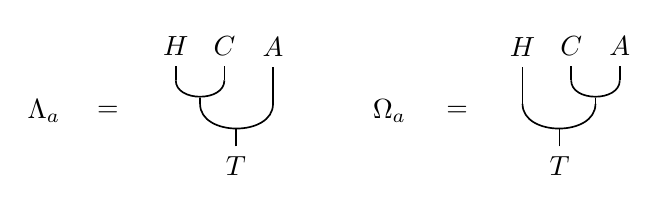
\begin{tikzpicture}[xscale = .65, yscale = .6, baseline=(current  bounding  box.center)]
\begin{pgfonlayer}{nodelayer}
		\node [style=none] (139) at (-1.625, 5.45) {};
		\node [style=none] (141) at (-1.625, 5.325) {};
		\node [style=none, label={above : $H$}] (144) at (-2.1, 6.125) {};
		\node [style=none] (146) at (-2.1, 5.825) {};
		\node [style=none] (246) at (-0.925, 4.8) {};
		\node [style=none, label={below : $T$}] (247) at (-0.925, 4.425) {};
		\node [style=none, label={above : $A$}] (249) at (-0.2, 6.1) {};
		\node [style=none] (250) at (-0.2, 5.325) {};
		\node [style=none, label={above : $C$}] (251) at (-1.15, 6.125) {};
		\node [style=none] (252) at (-1.15, 5.825) {};
		\node [style=none] (281) at (3.4, 5.175) {$=$};
		\node [style=none] (298) at (6.1, 5.45) {};
		\node [style=none] (299) at (6.1, 5.325) {};
		\node [style=none, label={above : $A$}] (300) at (6.575, 6.125) {};
		\node [style=none] (301) at (6.575, 5.825) {};
		\node [style=none] (302) at (5.4, 4.8) {};
		\node [style=none, label={below : $T$}] (303) at (5.4, 4.425) {};
		\node [style=none, label={above : $H$}] (304) at (4.675, 6.1) {};
		\node [style=none] (305) at (4.675, 5.325) {};
		\node [style=none, label={above : $C$}] (306) at (5.625, 6.125) {};
		\node [style=none] (307) at (5.625, 5.825) {};
		\node [style=none] (338) at (-3.425, 5.175) {$=$};
		\node [style=none] (339) at (-4.675, 5.175) {$\Lambda_a$};
		\node [style=none] (340) at (2.075, 5.175) {$\Omega_a$};
	\end{pgfonlayer}
	\begin{pgfonlayer}{edgelayer}
		\draw [style=wire] (141.center) to (139.center);
		\draw [style=wire] (146.center) to (144.center);
		\draw [style=wire] (247.center) to (246.center);
		\draw [style=wire] (250.center) to (249.center);
		\draw [style=wire] (252.center) to (251.center);
		\draw [style=wire, bend right=90, looseness=1.25] (141.center) to (250.center);
		\draw [style=wire, bend right=90, looseness=1.25] (146.center) to (252.center);
		\draw [style=wire] (299.center) to (298.center);
		\draw [style=wire] (301.center) to (300.center);
		\draw [style=wire] (303.center) to (302.center);
		\draw [style=wire] (305.center) to (304.center);
		\draw [style=wire] (307.center) to (306.center);
		\draw [style=wire, bend left=90, looseness=1.25] (299.center) to (305.center);
		\draw [style=wire, bend left=90, looseness=1.25] (301.center) to (307.center);
	\end{pgfonlayer}
\end{tikzpicture}
\end{equation}
where the subscript ``$a$'' indicates the element in the alphabet $S$ as well as the corresponding duplicate in question, the ordering on the output of each node is given from left to right,  and the uppercase letters indicate what the bijections $\alpha$, $\beta$ are (we use letters instead of numerals to avoid unintended orderings). For left counitality,
\begin{equation}\label{temp:counit}
\begin{tikzpicture}[xscale = .65, yscale = .4, baseline=(current  bounding  box.center)]
\begin{pgfonlayer}{nodelayer}
		\node [style=none] (314) at (8.7, 5.675) {$=$};
		\node [style=none, label={above : $H$}] (316) at (4.5, 6.6) {};
		\node [style=none, label={below : $C$}] (317) at (4.5, 4.925) {};
		\node [style=none] (324) at (11.525, 6.5) {$\bullet$};
		\node [style=none] (325) at (11.525, 5.575) {};
		\node [style=none] (326) at (10.825, 5.05) {};
		\node [style=none, label={below : $C$}] (327) at (10.825, 4.425) {};
		\node [style=none, label={above : $H$}] (328) at (10.1, 6.6) {};
		\node [style=none] (329) at (10.1, 5.575) {};
		\node [style=none] (330) at (7.6, 5.675) {$\Omega_a$};
		\node [style=none] (331) at (2.15, 5.675) {$\Lambda_a$};
		\node [style=none] (332) at (3.15, 5.675) {$=$};
	\end{pgfonlayer}
	\begin{pgfonlayer}{edgelayer}
		\draw [style=wire] (317.center) to (316.center);
		\draw [style=wire] (325.center) to (324.center);
		\draw [style=wire] (327.center) to (326.center);
		\draw [style=wire] (329.center) to (328.center);
		\draw [style=wire, bend left=90, looseness=1.25] (325.center) to (329.center);
	\end{pgfonlayer}
\end{tikzpicture}
\end{equation}
where the dot indicates that the discard $\epsilon_a$ is assigned to the terminal node, similarly for right counitality. For cocommutativity,
\begin{equation}\label{temp:cocom}
\begin{tikzpicture}[xscale = .65, yscale = .4, baseline=(current  bounding  box.center)]
\begin{pgfonlayer}{nodelayer}
		\node [style=none] (314) at (9.2, 5.675) {$=$};
		\node [style=none, label={above : $H$}] (324) at (12.025, 6.625) {};
		\node [style=none] (325) at (12.025, 5.575) {};
		\node [style=none] (326) at (11.325, 5.05) {};
		\node [style=none, label={below : $A$}] (327) at (11.325, 4.425) {};
		\node [style=none, label={above : $C$}] (328) at (10.6, 6.6) {};
		\node [style=none] (329) at (10.6, 5.575) {};
		\node [style=none] (330) at (8.1, 5.675) {$\Omega_a$};
		\node [style=none] (331) at (2.15, 5.675) {$\Lambda_a$};
		\node [style=none] (332) at (3.15, 5.675) {$=$};
		\node [style=none, label={above : $C$}] (333) at (5.95, 6.625) {};
		\node [style=none] (334) at (5.95, 5.575) {};
		\node [style=none] (335) at (5.25, 5.05) {};
		\node [style=none, label={below : $A$}] (336) at (5.25, 4.425) {};
		\node [style=none, label={above : $H$}] (337) at (4.525, 6.6) {};
		\node [style=none] (338) at (4.525, 5.575) {};
	\end{pgfonlayer}
	\begin{pgfonlayer}{edgelayer}
		\draw [style=wire] (325.center) to (324.center);
		\draw [style=wire] (327.center) to (326.center);
		\draw [style=wire] (329.center) to (328.center);
		\draw [style=wire, bend left=90, looseness=1.25] (325.center) to (329.center);
		\draw [style=wire] (334.center) to (333.center);
		\draw [style=wire] (336.center) to (335.center);
		\draw [style=wire] (338.center) to (337.center);
		\draw [style=wire, bend left=90, looseness=1.25] (334.center) to (338.center);
	\end{pgfonlayer}
\end{tikzpicture}
\end{equation}
This may seem different from how cocommutativity is depicted in (\ref{mon:law}). As we have explained in Remark~\ref{free:sys:mo:string}, the crossing is an artifact of representing graphs on a plane and may be dispensed with if we spell out the orderings, which is all that really matters. Finally, for naturality of discard,
\begin{equation}\label{temp:discar}
\begin{tikzpicture}[xscale = .55, yscale = .5, baseline=(current  bounding  box.center)]
\begin{pgfonlayer}{nodelayer}
		\node [style=none] (314) at (7.525, 5.675) {$=$};
		\node [style=none, label={below : $1$}] (324) at (2.15, 5) {};
		\node [style=none] (325) at (2.15, 6.55) {$\bullet$};
		\node [style=none] (328) at (8.9, 6.075) {};
		\node [style=none] (329) at (8.9, 7.1) {$\bullet$};
		\node [style=none] (330) at (6.425, 5.675) {$\Omega_f$};
		\node [style=none] (331) at (-0.325, 5.675) {$\Lambda_f$};
		\node [style=none] (332) at (0.675, 5.675) {$=$};
		\node [style=none, label={below : $1$}] (337) at (8.9, 4.325) {};
		\node [style=none] (338) at (8.9, 5.35) {};
		\node [style=wide small box] (339) at (9.625, 5.75) {$f$};
		\node [style=none] (340) at (10.35, 6.075) {};
		\node [style=none] (341) at (10.35, 7.1) {$\bullet$};
		\node [style=none, label={below : $k$}] (342) at (10.35, 4.325) {};
		\node [style=none] (343) at (10.35, 5.35) {};
		\node [style=none] (344) at (9.625, 6.75) {$\cdots$};
		\node [style=none] (345) at (9.625, 4.7) {$\cdots$};
		\node [style=none, label={below : $k$}] (346) at (3.65, 5) {};
		\node [style=none] (347) at (3.65, 6.55) {$\bullet$};
		\node [style=none] (348) at (2.9, 5.75) {$\cdots$};
	\end{pgfonlayer}
	\begin{pgfonlayer}{edgelayer}
		\draw [style=wire] (325.center) to (324.center);
		\draw [style=wire] (329.center) to (328.center);
		\draw [style=wire] (338.center) to (337.center);
		\draw [style=wire] (341.center) to (340.center);
		\draw [style=wire] (343.center) to (342.center);
		\draw [style=wire] (347.center) to (346.center);
	\end{pgfonlayer}
\end{tikzpicture}
\end{equation}
where the subscript ``$f$'' indicates the arrow  in question and the numerals indicate the ordering on the input of $f$ as well as what the bijection $\alpha$ is (there is no need to depict $\beta$ as the graphs have the empty codomain). Here $f$ runs through all the arrows of $G$, the discards in $\Lambda_f$ are those on the letters of the source of $f$, and the discards in $\Omega_f$ are those on the letters of its target. The cases where the source or the target of $f$ is the empty word are included: in the former $\Lambda_f$ is empty, and in the latter $\Omega_f$ consists of the node $f$ and its inputs. We also include the empty template and the versions that switch the roles of $\Lambda$, $\Omega$ so that the set becomes symmetric. Denote the resulting monoidal congruence relation on $\cat F_s(G)$ by $\bm S_M$.


Let $a = a_1 \ldots a_n$ be an object in $\cat F_s(G)$, where $a_i \in S$. Let $\Gamma$ be the diagram that joins those of $\bigotimes_i \delta_{a_i}$, $(\bigotimes_i 1_{a_i}) \otimes (\bigotimes_i 1_{a_i})$ together by connecting, for each $i$, the two outputs of $\delta_{a_i}$ with the $i$th and the $(n+i)$th edges of the latter (it is not enough to match the values in $S$, since a letter may occur more than once in $a$). Of course $\Gamma$ is not unique, as the two outputs of each $\delta_{a_i}$ may be connected in either order. On the other hand, in light of (\ref{temp:cocom}), all such $\Gamma$ represent the same  morphism in the quotient category $\cat F_s(G) / \bm S_M$, which is denoted by $\delta_a$ (it is the identity if $a$ is the empty word). Also set $\epsilon_a = \bigotimes_i \epsilon_{a_i}$ in $\cat F_s(G) / \bm S_M$. We claim that the equalities (\ref{mon:law}), (\ref{fins:frob}), and (\ref{discar:nat}) hold in $\cat F_s(G) / \bm S_M$ for all objects and all morphisms, in other words, that $\cat F_s(G) / \bm S_M$ is a Markov category; it is strict since $\cat F_s(G)$ is.

For (\ref{fins:frob}), this is how $\delta_a$ and $\epsilon_a$ have been defined: if $a$, $b$ are words of lengths $n$, $m$ then $\delta_{ab}$ and $(1_a \otimes \sigma_{ab} \otimes 1_b) \circ (\delta_a \otimes \delta_b)$ are represented by the same diagram, in which the two outputs of the duplicate at the $i$th position are connected with the $i$th and the $(n + m + i)$th edges of the codomain, and $\epsilon_{ab} = \epsilon_a \otimes \epsilon_b$.

For (\ref{mon:law}), let $a = a_1 \ldots a_n$ as above. Each side of the coassociativity law for $\delta_a$ is represented by a diagram in which, for every $i$, the $i$th edge of the domain enters a duplicate on $a_i$, one output of which enters a second duplicate on $a_i$, and the three remaining outputs are connected with the $i$th, the $(n + i)$th, and the $(2n + i)$th edges of the codomain. At each $i$ the two diagrams differ as the two sides of (\ref{temp:coass}) do, so $n$ Markov surgeries take one to the other. Similarly, $n$ surgeries with (\ref{temp:counit}) take a diagram representing $(\epsilon_a \otimes 1_a) \circ \delta_a$ to the one representing $1_a$, and likewise on the other side. Finally, $\sigma_{aa} \circ \delta_a$ is represented by one of the diagrams $\Gamma$ above, and hence equals $\delta_a$.

For (\ref{discar:nat}), we need to show that $\epsilon_c \circ [\Gamma] = \epsilon_b$ in $\cat F_s(G) / \bm S_M$ for every anchored diagram $\Gamma$ in $G$ from a word $b$ to a word $c$. Let $\Gamma^{\epsilon}$ be the diagram obtained from $\Gamma$ by ending each edge in $\cod(\Gamma)$ at a new node that carries the discard in question; it represents $\epsilon_c \circ [\Gamma]$ and does not depend on the ordering of $\cod(\Gamma)$. We proceed by induction on the number of inner nodes of $\Gamma$. If there is none then $\Gamma$ consists of loose edges and $\Gamma^{\epsilon}$ represents $\epsilon_b$. Otherwise let $x$ be a maximal element of $\dot \Gamma$, so that all the edges in $\out(x)$ belong to $\cod(\Gamma)$, and let $f$ be the arrow of $G$ assigned to $x$. In $\Gamma^{\epsilon}$, the node $x$, the discards on its outputs, and all the edges at these nodes form a subgraph that is isomorphic to $\Omega_f$ in (\ref{temp:discar}). This subgraph is normal: it has no loose edges, it contains all the edges at its nodes, and the directed paths between its nodes are the outputs of $x$. The surgery that replaces it with $\Lambda_f$ results in $\Upsilon^{\epsilon}$, where $\Upsilon$ is obtained from $\Gamma$ by removing $x$ and its outputs, so that the inputs of $x$ now belong to the codomain. Since $\Upsilon$ has the same domain as $\Gamma$ and one inner node fewer, $\Upsilon^{\epsilon}$ represents $\epsilon_b$ in $\cat F_s(G) / \bm S_M$ by the inductive hypothesis, and hence so does $\Gamma^{\epsilon}$.

Let $i_s : G \fun \cat F_s(G)$ be the obvious graph monoid homomorphism (see the proofs of \cite[Theorems~1.2, 2.3]{joyal1991geometry} for details); note that either one of the diagrams in (\ref{temp:cocom}) may be designated as the duplicate on $a$ in $\cat F_s(G)$, but the choice is manifestly unnatural, so we do not treat $i_s$ as a graph monoid homomorphism matching duplicates and discards. On the other hand,
\[
i_m = (- / \bm S_M ) \circ i_s: G \fun \cat F_s(G) / \bm S_M
\]
is a graph monoid homomorphism matching duplicates and discards.

Now, let $\cat D$ be a strict Markov category and $f : G \fun  \cat D$ a graph monoid homomorphism matching duplicates and discards. By Theorem~\ref{free:sym} and the sentence after it, there is exactly one strict symmetric monoidal functor
\[
F_s : \cat F_s(G) \fun \cat D \quad \text{with} \quad f = F_s \circ i_s.
\]
Since $f$ matches duplicates and discards, $F_s$ sends the two diagrams of each Markov template to the two sides of an instance of one of the equalities (\ref{mon:law}), (\ref{discar:nat}) in $\cat D$; for (\ref{temp:discar}) we also use the second equality in (\ref{fins:frob}), by which the discard on a product in $\cat D$ is the product of the discards. So $F_s$ takes the same value on the two diagrams. The pairs of morphisms on which $F_s$ takes the same value form a monoidal congruence relation on $\cat F_s(G)$, and hence, by Corollary~\ref{graph:small}, we must have $F_s([\Upsilon]) = F_s([\Gamma])$ if $[\Upsilon] /  \bm S_M =  [\Gamma] /  \bm S_M$. This yields a strict symmetric monoidal functor $F_m : \cat F_s(G) /  \bm S_M \fun \cat D$ with $F_s = F_m \circ (- / \bm S_M)$ and hence $f = F_m \circ i_m$. It is a Markov functor: it matches the duplicates and the discards on the letters because $f$ does, and then on all words because, by (\ref{fins:frob}), those on a word are expressed in the same way through those on its letters in $\cat F_s(G) /  \bm S_M$ and in $\cat D$. It is the only strict Markov functor with $f = F_m \circ i_m$: if $F'$ is another one then $F' \circ (- / \bm S_M)$ is a strict symmetric monoidal functor with $f = F' \circ (- / \bm S_M) \circ i_s$, so it equals $F_s$, and $- / \bm S_M$ is surjective on objects and on morphisms. In summary, we have a commutative diagram
\begin{equation}\label{free:mark:dia}
  \bfig
      \Vtrianglepair(0,0)/<-`->`<-`<-`<-/<700,400>[\cat F_s(G) / \bm S_M`\cat F_s(G)`\cat D`G; - / \bm S_M`F_s`i_m`i_s`f]
      \morphism(0,400)|a|/{@{->}@/^3em/}/<1400,0>[\phantom{\cat F_s(G) / \bm S_M}`\phantom{\cat D};F_m]
  \efig
\end{equation}
In conclusion, we have shown:

\begin{thm}\label{free:markov:quot}
The quotient category $\cat F_s(G) / \bm S_M$ is the free Markov category over $G$.
\end{thm}

More informatively, this means that the graphical language of  symmetric monoidal categories over $G$, with the additional syntax depicted in (\ref{mon:law}), (\ref{fins:frob}), and (\ref{discar:nat}), up to Markov surgeries  (instead of isomorphisms as in free symmetric monoidal categories and many other cases discussed in \cite{selinger2010survey}) forms the free  Markov category over $G$, which is strict. Note that $F_m$ in (\ref{free:mark:dia}) is unique, and not merely unique up to an isomorphism, because it is required to be strict; compare the remark after the proof of \cite[Theorem~1.2]{joyal1991geometry}.

\begin{rem}\label{graph:lan:mar}
In terms of coherence, freeness may be reformulated as follows. A well-formed
equation between morphisms in the symbolic language of symmetric monoidal categories
follows from the axioms of Markov categories if and only if it holds, up to Markov surgeries, in the graphical language of symmetric monoidal categories.
\end{rem}


A node $x$ of an anchored diagram $(\Gamma, v)$ in $G$ is \memph{quasi-terminal} if either it is terminal or every maximal directed path $p$ in $\Gamma$ with $p(0) = x$ ends at a terminal node or, in case that $v(x)$ is a duplicate, this is so for all such paths through one of the prongs.  Denote the set of quasi-terminal nodes of $\Gamma$ by $\Delta_\Gamma$ and its complement by  $\tilde \Delta_\Gamma = \Gamma_0 \mi \Delta_\Gamma$.

A \memph{splitter path} in $\Gamma$  is a  concatenation of two directed paths joined at the starting nodes, that is, a pair of directed paths $p$, $p'$ in $\Gamma$ with $p(0) = p'(0)$.

For an edge $e$ of $\Gamma$, its \memph{origin} $e^{\circ}$ is the edge obtained by following $e$ backward through the duplicates: if $e(0)$ is a node with $v(e(0))$ a duplicate then $e^{\circ} = e'^{\circ}$, where $e'$ is the input of $e(0)$, and otherwise $e^{\circ} = e$. This is well defined because there are no directed circuits. So $e^{\circ}$ is either an edge in $\dom(\Gamma)$ or an output of a node whose value is not a duplicate.

A node $x$ of $\Gamma$ is \memph{live} if $x \in \tilde \Delta_\Gamma$ and $v(x)$ is not a duplicate, in other words, if $v(x)$ is not a duplicate and there is a directed path $p$ in $\Gamma$ with $p(0) = x$ that ends in $\cod(\Gamma)$. An edge of $\Gamma$ is a \memph{consumer} if it belongs to $\cod(\Gamma)$ or is an input of a live node. The origin of a consumer is either an edge in $\dom(\Gamma)$ or an output of a live node. We say that two anchored diagrams $(\Gamma, v)$, $(\Upsilon, w)$ in $G$ with the same domain and the same codomain \memph{have the same skeleton} if there is a bijection $\pi$ from the set of the live nodes of $\Gamma$ onto that of $\Upsilon$ such that $v(x) = w(\pi(x))$ for all live $x$ and the origins match: if $e$ is the $i$th edge in $\cod(\Gamma)$, or the $i$th input of a live node $x$, and $e'$ is the $i$th edge in $\cod(\Upsilon)$, or the $i$th input of $\pi(x)$, respectively, then $e^{\circ}$ is the $j$th edge in $\dom(\Gamma)$ if and only if $e'^{\circ}$ is the $j$th edge in $\dom(\Upsilon)$, and $e^{\circ}$ is the $j$th output of a live node $y$ if and only if $e'^{\circ}$ is the $j$th output of $\pi(y)$.

\begin{lem}\label{decor:mat}
Suppose that $(\Gamma, v)$, $(\Upsilon, w)$ are anchored diagrams belonging to the same $\bm S_M$-congruence class. Then they have the same skeleton, say, via the bijection $\pi$. Consequently,
\begin{itemize}
 \item $\pi$ extends to a bijection $\tilde \Delta_\Gamma \fun \tilde \Delta_{\Upsilon}$ compatible with the valuations, that is, $v(x) = w(\pi(x))$ for all $x \in \tilde \Delta_\Gamma$;
 \item for all live nodes $x$, $y$ of $\Gamma$, there is a directed path in $\Gamma$ from $x$ to $y$ if and only if there is one in $\Upsilon$ from $\pi(x)$ to $\pi(y)$, and the same holds for the directed paths that begin with the $i$th edge in the domain instead of beginning at $x$, $\pi(x)$, or end with the $j$th edge in the codomain instead of ending at $y$, $\pi(y)$;
 \item the same holds for the splitter paths between two ends each of which is a live node or an edge in the codomain.
\end{itemize}
\end{lem}
\begin{proof}
Isomorphic diagrams have the same skeleton, so for the first claim it is enough to consider the case that $\Upsilon$ is the result of a Markov surgery on $\Gamma$, say, with the normal subgraph $\Gamma' \sub \Gamma$ and the template $(\Omega / \Lambda, \alpha, \beta)$. The nodes and the edges of $\Gamma$ outside $\Gamma'$ are also nodes and edges of $\Upsilon$, and the edges in $\dom(\Gamma')$, $\cod(\Gamma')$ are identified with those in $\dom(\Lambda)$, $\cod(\Lambda)$.

If the template is one of (\ref{temp:coass}), (\ref{temp:counit}), (\ref{temp:cocom}), in either direction, then the nodes of $\Omega$ and $\Lambda$ are duplicates and discards, so none of them is live, the domain of each of $\Omega$, $\Lambda$ is a single edge, and this edge is the origin, in $\Omega$ or $\Lambda$, of every edge in the codomain. Therefore a directed path in $\Gamma$ that ends in $\cod(\Gamma)$ and passes through $\Gamma'$ may be rerouted through $\Lambda$, and vice versa, so $\Gamma$ and $\Upsilon$ have the same live nodes; and following an edge backward through $\Gamma'$ or through $\Lambda$ leads to the same edge, so the consumers have the same origins in $\Gamma$ and in $\Upsilon$.

If the template is (\ref{temp:discar}), in either direction, then the codomains of $\Omega$ and $\Lambda$ are empty. So no directed path that ends in $\cod(\Gamma)$ or in $\cod(\Upsilon)$ contains a node or an edge of $\Gamma'$ or of $\Lambda$; in particular, no node of $\Gamma'$ or of $\Lambda$ is live, and no edge of them is a consumer or the origin of a consumer. Again $\Gamma$ and $\Upsilon$ have the same live nodes and the consumers have the same origins.

For the second item, let $p$ be a directed path in $\Gamma$ that begins at a live node or with an edge in $\dom(\Gamma)$ and ends at a live node or with an edge in $\cod(\Gamma)$. Since $p$ may be prolonged to a directed path that ends in $\cod(\Gamma)$, every node on it is live or a duplicate. So $p$ is a concatenation of consumers $e_1, \ldots, e_n$, each preceded by the edges that lead to it from its origin through duplicates, where the origin of $e_1$ is the first edge of $p$ and the origin of $e_{k+1}$ is an output of the live node $e_k(1)$ for $k < n$. Conversely, every such sequence of consumers gives a directed path. Since the skeleton records exactly the origins of the consumers, the second item follows.

For the third item, let $p$, $p'$ form a splitter path between such ends. If $p(0) = p'(0)$ is a duplicate then let $q$ be the origin of its input; prolonging $p$, $p'$ backward to $q$, we may assume that they begin with the same edge in $\dom(\Gamma)$ or at the same node, which is live as before. Now apply the second item to $p$ and to $p'$.

For the first item, a node in $\tilde \Delta_\Gamma$ whose value is not a duplicate is live. Let $d$ be a node whose value is a duplicate and $q$ the origin of its input. The edges with the origin $q$ form a tree that branches at duplicates, and $d \in \tilde \Delta_\Gamma$ if and only if through each of the two outputs of $d$ there is a directed path that ends in $\cod(\Gamma)$, that is, if and only if each of the two branches at $d$ contains a consumer. So, if $n \geq 1$ is the number of the consumers with the origin $q$, then exactly $n - 1$ duplicates in this tree belong to $\tilde \Delta_\Gamma$, and their value is the duplicate on $v(q)$. Since $n$ is determined by the skeleton, $\pi$ may be extended as required.
\end{proof}

The three items are the properties of diagrams used in \cite{yinzhang2021}. Note that the second and the third ones concern the existence of a path between given ends, not the number of such paths or the nodes on them, which may change under a surgery with (\ref{temp:coass}).

Call the diagram $\Gamma$ \memph{Markov minimal} if the value of every node in $\Delta_\Gamma$ is a discard; in that case, surgeries with the templates  (\ref{temp:counit}), (\ref{temp:discar}) can no longer be applied in the $\Omega$-to-$\Lambda$ direction, except for those with (\ref{temp:discar}) where $f$ is itself a discard, which do not change the diagram. Compare the normalized diagrams of \cite[Definition~6.2]{FriLiang2022}.

We say that $\Upsilon$ is \memph{Markov congruent} to $\Gamma$ if they become isomorphic upon surgeries with the templates (\ref{temp:coass}), (\ref{temp:cocom}).

\begin{lem}\label{mar:min:com}
Every $\bm S_M$-congruence class contains a Markov minimal diagram, and any two Markov minimal diagrams with the same skeleton are Markov congruent. Consequently, two anchored diagrams in $G$ with the same domain and the same codomain belong to the same $\bm S_M$-congruence class if and only if they have the same skeleton, and any two Markov minimal diagrams in the same $\bm S_M$-congruence class are Markov congruent.
\end{lem}
\begin{proof}
For the first claim, suppose that $\Gamma$ is not Markov minimal. We show that a Markov surgery on $\Gamma$ results in a diagram with fewer nodes whose values are not discards, which is enough. Let $x$ be maximal in $\dot \Gamma$ among the nodes in $\Delta_\Gamma$ whose values are not discards. If $y$ is the target of an output $e$ of $x$ and all the maximal directed paths that start at $x$ and contain $e$ end at terminal nodes then $y \in \Delta_\Gamma$, and hence $v(y)$ is a discard by the choice of $x$. So, if $v(x)$ is a duplicate then one of its outputs ends at a discard, and a surgery with (\ref{temp:counit}) removes $x$ and this discard. If $v(x) = f$ is not a duplicate then all the outputs of $x$, if any, end at discards, and a surgery with (\ref{temp:discar}) replaces $x$ and these discards with discards on the inputs of $x$.

For the second claim, let $\Gamma$ be Markov minimal. Then a node of $\Gamma$ is either live or a duplicate in $\tilde \Delta_\Gamma$ or a discard. Let $q$ be an edge in $\dom(\Gamma)$ or an output of a live node, and consider the edges with the origin $q$. They form a tree with the root $q$ that branches at duplicates, and each of its leaves is a consumer or ends at a discard. If the tree contains a duplicate then no leaf ends at a discard, because a duplicate with an output ending at a discard is in $\Delta_\Gamma$. So either no consumer has the origin $q$ and $q$ itself ends at a discard, or the tree is a binary tree of duplicates whose leaves are the consumers with the origin $q$. Conversely, the input of a discard is not an output of a duplicate, and hence it is such an edge $q$. This shows that $\Gamma$ is determined, up to isomorphisms, by its skeleton and the shapes of these trees.

Now, any two binary trees of duplicates with the same leaves may be transformed into each other by surgeries with (\ref{temp:coass}), (\ref{temp:cocom}). Indeed, this is clear if there are at most two leaves. In general, a leaf at a duplicate $d$ other than the root may be moved to the duplicate that precedes $d$ by a surgery with (\ref{temp:coass}), after surgeries with (\ref{temp:cocom}) if necessary; so both trees may be transformed so that a given leaf is at the root, and we conclude by induction on the number of leaves. The second claim follows.

The remaining claims follow from the first two and Lemma~\ref{decor:mat}.
\end{proof}

We record one more consequence of the last two lemmas, which is also used in \cite{yinzhang2021}.

\begin{lem}\label{dead:inp}
Let $(\Gamma, v)$ be an anchored diagram in $G$ from a word $a = a_1 \ldots a_n$ to a word $b$. Let $J$ be the set of those $j$ such that the $j$th edge in $\dom(\Gamma)$ is not the origin of a consumer, $a'$ the subword of $a$ at the positions in $J$, and $a''$ the subword of $a$ at the other positions. Then
\begin{itemize}
 \item $j \notin J$ if and only if there is a directed path in $\Gamma$ that begins with the $j$th edge in $\dom(\Gamma)$ and ends in $\cod(\Gamma)$;
 \item the set $J$ is the same for all the diagrams in the $\bm S_M$-congruence class of $\Gamma$;
 \item there is a unique morphism $g : a'' \fun b$ in $\cat F_s(G) / \bm S_M$ such that $[\Gamma] / \bm S_M = (g \otimes \epsilon_{a'}) \circ \tau$, where $\tau : a \fun a''a'$ is the symmetry that moves the letters at the positions in $J$ to the end and does not change the order of the other letters or that of the letters moved; moreover, in every diagram that represents $g$, every edge in the domain begins a directed path that ends in the codomain.
\end{itemize}
\end{lem}
\begin{proof}
Let $e$ be the $j$th edge in $\dom(\Gamma)$. If $e$ is the origin of a consumer $e'$ then the edges that lead from $e$ to $e'$ through duplicates form a directed path, and either $e' \in \cod(\Gamma)$ or $e'$ is an input of a live node, from which a directed path leads to $\cod(\Gamma)$. Conversely, let $p$ be a directed path that begins with $e$ and ends in $\cod(\Gamma)$. Every node on $p$ whose value is not a duplicate is live. So the first edge on $p$ that belongs to $\cod(\Gamma)$ or is an input of such a node is a consumer, and its origin is $e$. This proves the first item. The second item follows from Lemma~\ref{decor:mat}, since the skeleton records which edges in the domain are origins of consumers.

For the third item, by Lemma~\ref{mar:min:com} and the second item, we may assume that $\Gamma$ is Markov minimal. Let $j \in J$ and $e$ be as above. Then $e \notin \cod(\Gamma)$ and, by the first item, no directed path that starts at the node $e(1)$ ends in $\cod(\Gamma)$. So $e(1) \in \Delta_\Gamma$ and hence its value is a discard. Removing these edges and discards for all $j \in J$, we obtain an anchored diagram $\Gamma''$ from $a''$ to $b$, and $g = [\Gamma''] / \bm S_M$ is as required. The live nodes and the consumers of $\Gamma''$ are those of $\Gamma$, so every edge in $\dom(\Gamma'')$ is the origin of a consumer, and the last claim follows from the first two items applied to $\Gamma''$. If $g'$ is another such morphism and $\Upsilon$ is a diagram that represents it then the diagram obtained from $\Upsilon$ by adding, for each $j \in J$, an edge that ends at a discard as the $j$th edge in the domain is in the $\bm S_M$-congruence class of $\Gamma$ and has the same live nodes and consumers as $\Upsilon$. By Lemma~\ref{decor:mat}, it has the same skeleton as $\Gamma$, and hence $\Upsilon$ has the same skeleton as $\Gamma''$. So $g' = g$ by Lemma~\ref{mar:min:com}.
\end{proof}




\section{Effects in a Markov category}

Generalizing the construction of a causal conditional in \cite[\S~4]{Fong:thesis}, we shall define a class of morphisms in an arbitrary Markov category $\cat M$ that will be of central interest.

We first assume that $\cat M$ is \memph{straight}; this just means that $\cat M$ is strict and the monoid $(\cat M_0, \otimes, \moi)$ has no idempotents or elements of finite order  other than $\moi$; these two conditions are met in many natural situations where the results of this paper are intended for application.  Note that the second condition holds if and only if $w^n \neq w^m$ for all $w \neq \moi$ and all $n \neq m > 0$; here $w^n$ is a shorthand for  the  monoidal product of $n$ copies of $w$ itself; this includes the empty product $w^0 = \moi$.



\begin{defn}
Let $W = ( w_1, \ldots, w_n )$ be a sequence of objects  and $w = \bigotimes_i w_i$. A morphism $w \fun v$ in $\cat M$ is called a \memph{multiplier} on $(W, v)$  if it is generated from the duplicates, discards, symmetries, and identities on $w_i$, $1 \leq i \leq n$.
\end{defn}

\begin{rem}\label{mul:pow}
If $n = 1$ then there is exactly one multiplier on $(w, w^m)$, which is denoted by $\iota_{w \rightarrow w^m}$. So $\iota_{w \rightarrow \moi} = \epsilon_w$, $\iota_{w \rightarrow w} = 1_w$, $\iota_{w \rightarrow w^2} = \delta_w$, and $\iota_{w \rightarrow w^{m+1}} = (\iota_{w \rightarrow w^m} \otimes 1_w) \circ \delta_w$ for $m \geq 1$.

The uniqueness follows from the straightness of $\cat M$ and Lemma~\ref{mar:min:com}. This is clear if $w = \moi$, since $\moi$ is terminal. So assume $w \neq \moi$. Let $G_a$ be the free $\DD$-graph monoid with one letter $a$ whose only arrows are the duplicate and the discard on $a$ and, by Theorem~\ref{free:markov:quot}, let $F : \cat F_s(G_a) / \bm S_M \fun \cat M$ be the strict Markov functor with $F(a) = w$. Since $\cat M$ is straight, $w^k = w^l$ only if $k = l$. So, if $F(h) : w^k \fun w^l$ and $F(h') : w^{k'} \fun w^{l'}$ are composable in $\cat M$ then $h$ and $h'$ are composable in $\cat F_s(G_a) / \bm S_M$. Since the duplicate, the discard, the symmetry, and the identity on $w$ are in the image of $F$, it follows that every morphism generated from them by composition and monoidal product is in the image of $F$; in particular, every multiplier on $(w, w^m)$ is of the form $F(h)$ with $h : a \fun a^m$. Now, a diagram in $G_a$ from $a$ to $a^m$ has no live nodes, and the origin of every edge in its codomain is the edge in its domain. So any two such diagrams have the same skeleton, and hence there is only one morphism $a \fun a^m$ by Lemma~\ref{mar:min:com}.

The multiplier $\iota_{w \rightarrow w^m}$ may be depicted as a diagram in $\cat M$ that contains exactly one terminal node when $m = 0$, no node when $m = 1$, and $i$ nodes for any $1 \leq i \leq m - 1$ when $m > 1$, where each node has one input and $k \geq 2$ outputs and its value is $\iota_{w \rightarrow w^k}$, and where $i$ is chosen to be conducive to the situation at hand; by the uniqueness, all these diagrams represent the same morphism. The diagram in binary form is the one with $i = m - 1$, in which the value of every node is $\delta_w$. It is this form that is meant whenever nodes are counted, paths are compared, or the notions of \S~4 are applied to the diagram.
\end{rem}

\begin{rem}\label{uni:pro}
Suppose that $(\cat M_0, \otimes, \moi)$ is indeed a free monoid. Then the underlying graph monoid of $\cat M$ is a free $\DD$-graph monoid, with the duplicates and the discards on the letters, so the notions of \S~4 apply to the diagrams in it, and, by Theorem~\ref{free:markov:quot}, the diagrams in the same $\bm S_M$-congruence class represent the same morphism of $\cat M$.

If every $w_i$ is in the alphabet, $w_i \neq w_j$ for all $i \neq j$, and $v$ is a word in the letters $w_1, \ldots, w_n$ then there is again exactly one multiplier on $(W, v)$, which is denoted by $\iota_{w \rightarrow v}$; if another letter occurs in $v$ then there is no multiplier on $(W, v)$ at all. For the existence, take the monoidal product of the multipliers $\iota_{w_i \rightarrow w_i^{m_i}}$, where $m_i$ is the number of the occurrences of $w_i$ in $v$, followed by a symmetry that arranges the letters as in $v$. The uniqueness is shown as in Remark~\ref{mul:pow}, with $G_a$ replaced by the free $\DD$-graph monoid with $n$ letters $a_1, \ldots, a_n$ whose only arrows are the duplicates and the discards, and with $F(a_i) = w_i$: the functor $F$ is injective on objects since the $w_i$ are distinct letters, so composable morphisms in its image come from composable morphisms; a diagram from $a_1 \ldots a_n$ has no live nodes, and the origin of an edge in its codomain is the edge in its domain with the same value. For instance, if  $w = w_1 w_2 w_3$ and $v = w_1^2  w_2   w_1  w_2$ then $\iota_{w \rightarrow v}$ may be depicted as the Markov minimal diagram
$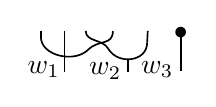
\begin{tikzpicture}[xscale = .3, yscale = .3, baseline={([yshift=8pt]current bounding box.south)}]
\begin{pgfonlayer}{nodelayer}
		\node [style=none] (108) at (4.275, 0.15) {};
		\node [style=none] (110) at (7.325, 0.15) {};
		\node [style=none] (111) at (5.275, -1.575) {};
		\node [style=none] (112) at (4.275, -0.1) {};
		\node [style=none] (113) at (6.275, -0.65) {};
		\node [style=none] (114) at (5.275, -0.95) {};
		\node [style=none] (117) at (6.175, 0.15) {};
		\node [style=none] (118) at (8.8, 0.15) {};
		\node [style=none] (119) at (7.975, -1.575) {};
		\node [style=none] (120) at (7.125, -0.6) {};
		\node [style=none] (121) at (8.775, -0.35) {};
		\node [style=none] (122) at (7.975, -1.075) {};
		\node [style=none] (124) at (10.2, -1.55) {};
		\node [style=none] (150) at (10.2, 0.025) {$\bullet$};
		\node [style=none] (151) at (5.275, 0.15) {};
		\node [style=none] (152) at (4.4, -1.5) {$w_1$};
		\node [style=none] (153) at (7, -1.55) {$w_2$};
		\node [style=none] (154) at (9.2, -1.5) {$w_3$};
	\end{pgfonlayer}
	\begin{pgfonlayer}{edgelayer}
		\draw [style=wire, in=-135, out=-90] (112.center) to (113.center);
		\draw [style=wire] (108.center) to (112.center);
		\draw [style=wire, in=45, out=-90, looseness=1.25] (110.center) to (113.center);
		\draw [style=wire, in=270, out=90] (111.center) to (114.center);
		\draw [style=wire, in=-90, out=-60, looseness=1.25] (120.center) to (121.center);
		\draw [style=wire, in=120, out=-90] (117.center) to (120.center);
		\draw [style=wire, in=90, out=-90, looseness=1.25] (118.center) to (121.center);
		\draw [style=wire] (119.center) to (122.center);
		\draw [style=wire] (124.center) to (150.center);
		\draw [style=wire] (114.center) to (151.center);
	\end{pgfonlayer}
\end{tikzpicture}$, where how the  duplicates in the trident are arranged, how the edges at the nodes are ordered, how the copies of the same object in the codomain are ordered, and so on, can all be left unspecified without any ambiguity.

If $w_i = w_j$ for some $i \neq j$ then multipliers may not be unique. In fact, this is so even if $w_i \neq w_j$ for all $i \neq j$, because there may be ``algebraic relations'' among $w_i$, $1 \leq i \leq n$, for example, $w_1w_2 = w_3$, unless every $w_i$ is in the alphabet, which then is the situation just discussed.
\end{rem}


A \memph{loop} in a directed graph  $G = (V(G), A(G), s, t)$ is an arrow in  $A(G)$ whose source and target coincide. Note that  $G$ could still be acyclic even if it has loops, because a cycle in $G$ does not contain loops by definition.  We shall work with directed graphs $G$ such that there is exactly one loop at each vertex in $G$, which is referred to as the \memph{identity loop} on $v$ and is denoted by $1_v$, for reasons that will become clear. The identity loops are disregarded whenever we speak of the parents or the children of a vertex, and a directed path, like a cycle, does not contain loops; so a vertex is neither a parent nor a child of itself.


The category \cat{FinDAG} has finite directed acyclic graphs with identity loops as objects and graph homomorphisms between them as morphisms.


We have a more flexible notion of morphisms in \cat{FinDAG}, because  arrows can be collapsed due to the presence of identity loops. For instance, under the standard definition, there can be no morphisms from any directed graph with a nonempty set of arrows to the directed graph with exactly one vertex; on the other hand, the one-vertex graph is the terminal object in \cat{FinDAG} as defined above, that is, every object in \cat{FinDAG} comes with exactly one morphism to it.

\begin{defn}\label{gen:condi}
Let $W = (w_1, \ldots, w_n)$ be a sequence of objects (repetitions are allowed, and so is $w_i = \moi$). For each $S \sub \{1, \ldots, n\}$, let $w_S = {\bigotimes_{i \in S}}  w_i$, taken in the increasing order of $i$, where $w_\0 = \moi$. For each $i$, let $S_i \sub \{1, \ldots, n\}$ with $i \notin S_i$ and $\kappa_{i} : w_{S_i} \fun w_i$ a morphism; let $K$ be the family of the pairs $(S_i, \kappa_i)$, $1 \leq i \leq n$. The sets $S_i$ are part of the data, since they cannot be recovered from the morphisms $\kappa_i$ if $w_j = w_k$ for some $j \neq k$. We associate a directed graph $G$ with $K$: the set $V(G)$ of vertices is $\{1, \ldots, n\}$  and there is an arrow $j  \rightarrow i$ if and only if  $j \in S_i$. Of course $G$ may or may not be cyclic. After adding identity loops, we do assume $G \in \cat{FinDAG}$. Among other things, this implies $S_i = \0$ for some $i$; in that case, $\kappa_i$ shall be depicted as $\begin{tikzpicture}[xscale = .3, yscale = .3, baseline={([yshift=6pt]current bounding box.south)}]
\begin{pgfonlayer}{nodelayer}
		\node [style=none] (124) at (9.825, -1.55) {$\bullet$};
		\node [style=none] (150) at (9.825, 0.025) {};
	\end{pgfonlayer}
	\begin{pgfonlayer}{edgelayer}
		\draw [style=wire] (124.center) to (150.center);
	\end{pgfonlayer}
\end{tikzpicture}$.

Let $S, T \sub V(G)$. Let $G_{S \rightarrow T}$ be the subgraph of $G$ that consists of all the vertices in $S \cup T$ and all the directed paths that end  in $T$ but do not \memph{travel toward} $S$, that is, do not pass through or end in $S$ (starting in $S$ is allowed). Note that, for every  $i \in V(G_{S \rightarrow T})$, if $i \notin S$ then its parents in $G$ are all in $G_{S \rightarrow T}$ as well and if $i \in S$ then it has no parents in $G_{S \rightarrow T}$.

Construct a diagram in $\cat M$  as follows. For each $i \in V(G_{S \rightarrow T})$, let $\bar w_i$ be the monoidal product of as many copies of $w_i$ as the number of children of $i$ in $G_{S \rightarrow T}$, that is, of those $k \in V(G_{S \rightarrow T}) \mi S$ with $i \in S_k$ (the identity loops are disregarded). Let $\stri_i$ be a  diagram of
\[
\begin{dcases*}
   \iota_{w_i \rightarrow \bar w_i w_i}                & if $i \in S \cap T$,\\
   \iota_{w_i \rightarrow \bar w_i}                            & if $i \in S \mi T$,\\
  \iota_{w_i \rightarrow \bar w_i w_i} \circ \kappa_i  & if $i \in T \mi S$,\\
  \iota_{w_i \rightarrow \bar w_i} \circ \kappa_i              & if $i \notin S \cup T$,
\end{dcases*}
\]
where in the last two cases the diagram for $\kappa_i$ is the obvious one, with a single node whose inputs correspond, in the increasing order, to the elements of $S_i$; note the extra copy of $w_i$ in the codomain of $\iota_{w_i \rightarrow \bar w_i w_i}$. So the domain of $\stri_i$ consists of one edge if $i \in S$ and of one edge for each $j \in S_i$ if $i \notin S$, and its codomain consists of one edge for each child of $i$ in $G_{S \rightarrow T}$ and, if $i \in T$, one more edge. For each $j \in V(G_{S \rightarrow T})$, assign the edges in the codomain of $\stri_j$, except one of them if $j \in T$, bijectively to the children of $j$ in $G_{S \rightarrow T}$, and identify the edge assigned to a child $i$ with the edge in the domain of $\stri_i$ that corresponds to $j \in S_i$. It is not enough to match the values of the edges, since $w_j = w_k$ may hold for $j \neq k$. This fuses the \memph{components} $\stri_i$ together into a single  diagram, denoted by $\stri_{[w_T \| w_S]_{(W, K)}}$. Its domain consists of the edges in the domains of $\stri_i$, $i \in S$, and its codomain consists of the remaining edges in the codomains of $\stri_j$, $j \in T$, both in the increasing order of the indices; so they are $w_S$ and $w_T$.

The diagram thus obtained is not unique up to isomorphisms, since the edges in the codomain of a multiplier may be assigned in any way. But the morphism that it represents is unique: by Remark~\ref{mul:pow}, the multipliers used here are unique, and changing an assignment amounts to composing a multiplier $\iota_{w_j \rightarrow w_j^m}$ with a symmetry, which gives a multiplier on $(w_j, w_j^m)$ again, that is, the same morphism. It is referred to as the \memph{$(W, K)$-effect} of $w_S$ on $w_T$ and is denoted by $[w_T \| w_S]_{(W, K)} : w_S \fun w_T$, or simply $[w_T]_{(W, K)}$ when $S = \0$.

If $(\cat M_0, \otimes, \moi)$ is a free monoid and every $w_i$ is in the alphabet then, with the multipliers in binary form, $\stri_{[w_T \| w_S]_{(W, K)}}$ is a diagram in the underlying free $\DD$-graph monoid of $\cat M$ (see Remark~\ref{uni:pro}). It is Markov minimal: each node with the value $\kappa_i$, $i \in V(G_{S \rightarrow T}) \mi S$, occurs once and is live, since a directed path leads from it to the codomain, and the other nodes are duplicates, none of which is quasi-terminal, and the discards on $w_j$ for those $j \in S \mi T$ without children. Any two such diagrams have the same skeleton, and hence are Markov congruent by Lemma~\ref{mar:min:com}.
\end{defn}

We shall write $[w_T \| w_S]$ simply as $[T \| S]$ when the context is clear. The subscript $(W, K)$ may be dropped from the notation too.

\begin{lem}\label{graph:split}
Let $i \in V(G_{S \rightarrow T}) \mi S$. Let $A$ be the set of the ancestors of $i$ in $G_{S \rightarrow T}$ (vertices are ancestors of themselves) and
\[
T_i = (A \cap T) \cup \{ j \in A : j \text{ has a child in } G_{S \rightarrow T} \text{ outside } A \} \cup (S \mi A).
\]
Then
\begin{itemize}
  \item $i \in T_i$ and $V(G_{S \rightarrow T_i})$ does not contain any child of $i$ in $G_{S \rightarrow T}$,
  \item $[T \| S] = [T \| T_i] \circ [T_i \| S]$; more precisely, if the multipliers are depicted suitably then there is a level $L$ of $\stri_{[T \| S]}$ such that $\stri_{[T \| S]}[\0, L] = \stri_{[{T_i} \| S]}$ and $\stri_{[T \| S]}[L, \dot \stri_{[T \| S]}] = \stri_{[{T} \| {T_i}]}$.
\end{itemize}
\end{lem}
\begin{proof}
Write $D = G_{S \rightarrow T}$. Recall that a vertex of $D$ outside $S$ has all its parents in $D$ and a vertex in $S$ has none. Since $i \notin S$, either $i \in T$ or $i$ has a child in $D$, and no child of $i$ is in $A$ because $D$ is acyclic; so $i \in T_i$.

We claim that $V(G_{S \rightarrow T_i}) = S \cup A$ and that the arrows of $G_{S \rightarrow T_i}$ are the arrows of $D$ that end in $A \mi S$. Indeed, from every vertex in $A \mi S$ a directed path in $D$ leads to $i \in T_i$. Conversely, a directed path that ends in $T_i$ and does not travel toward $S$ ends in $A \mi S$, and so all its vertices are in $D$ and are ancestors of $i$. In particular, the first item holds, since a child of $i$ in $D$ is neither in $A$ nor in $S$.

Next, we claim that $V(G_{T_i \rightarrow T}) = T_i \cup B$, where $B = V(D) \mi (A \cup S)$, and that the arrows of $G_{T_i \rightarrow T}$ are the arrows of $D$ that end in $B$. Indeed, from every vertex $k \in B$ a directed path in $D$ leads to $T$, and no vertex on it is in $S$ or, since $k \notin A$, in $A$; so it does not travel toward $T_i$. Conversely, let $p$ be a directed path that ends in $T$ and does not travel toward $T_i$. Since $T \cap (A \cup S) \sub T_i$, it ends in $B$. If $y \in B$ is a vertex on $p$ and $x$ is the vertex before it then $x \in V(D)$; if $x \in A$ then $x \in T_i$ because it has the child $y$ outside $A$, and if $x \in S \mi A$ then $x \in T_i$ as well. So either $x \in B$ or $x \in T_i$, and in the latter case $x$ is the first vertex on $p$. Finally, $T \sub T_i \cup B$.

So the set $V(D) \mi S$ is the disjoint union of $A \mi S$ and $B$, and, for every $j \in V(D)$, the children of $j$ in $D$ are its children in $G_{S \rightarrow T_i}$, which are those in $A$, together with its children in $G_{T_i \rightarrow T}$, which are those in $B$ and exist only if $j \in T_i \cup B$. Connect the codomain of $\stri_{[{T_i} \| S]}$ with the domain of $\stri_{[{T} \| {T_i}]}$. In the resulting diagram each $\kappa_j$, $j \in V(D) \mi S$, occurs once, and every edge in its domain comes from the vertex in $S_j$ to which it corresponds. For $j \in T_i$ the copies of $w_j$ are supplied by a multiplier of the first diagram, with one edge in its codomain for each child in $A$ and one more edge, followed by a multiplier of the second diagram, with one edge in its codomain for each child in $B$ and one more if $j \in T$. The composite of the two is a multiplier on $(w_j, w_j^m)$, where $m$ is the number of the children of $j$ in $D$, plus one if $j \in T$, and hence is $\iota_{w_j \rightarrow w_j^m}$ by Remark~\ref{mul:pow}. Therefore the resulting diagram is $\stri_{[T \| S]}$ with the multipliers on $w_j$, $j \in T_i$, depicted with two nodes, or with fewer if one of the two is an identity, and the nodes of $\stri_{[{T_i} \| S]}$ form the level $L$.
\end{proof}



\begin{prop}\label{mar:fun:eff}
Let $\cat N$ be another straight Markov category and $F : \cat M \fun \cat N$ a strict Markov functor. Let $F(W) = (F(w_1), \ldots, F(w_n))$ and let $F(K)$ be the family of the pairs $(S_i, F(\kappa_i))$, $1 \leq i \leq n$, so that the directed graph associated with $F(K)$ is $G$ again. Then
\[
F([T \| S]_{(W, K)}) = [T \| S]_{(F(W), F(K))}.
\]
\end{prop}
\begin{proof}
Let $(\Gamma, v)$ be a diagram $\stri_{[T \| S]_{(W, K)}}$ in $\cat M$. The morphism that it represents is obtained from the values of its nodes by compositions, monoidal products, and symmetries, see \cite[Chapter~2, \S~2]{joyal1991geometry}. Since $F$ is a strict symmetric monoidal functor, it sends this morphism to the one represented by $(\Gamma, F \circ v)$ in $\cat N$. Now, $F \circ v$ sends a node with the value $\kappa_i$ to $F(\kappa_i)$ and a node with the value $\iota_{w_j \rightarrow w_j^m}$ to $F(\iota_{w_j \rightarrow w_j^m})$. Since $F$ matches the duplicates and the discards and preserves symmetries and identities, the latter is a multiplier on $(F(w_j), F(w_j)^m)$, and hence equals $\iota_{F(w_j) \rightarrow F(w_j)^m}$ by Remark~\ref{mul:pow}, because $\cat N$ is straight. So $(\Gamma, F \circ v)$ is a diagram $\stri_{[T \| S]_{(F(W), F(K))}}$.
\end{proof}

More generally, we shall consider  \memph{twists} of $[T \| S]$. For a permutation $\tau$ of $T$, let $w_{\tau(T)}$ be the monoidal product of the objects $w_i$, $i \in T$, taken in the order $\tau(t_1), \ldots, \tau(t_m)$, where $t_1 < \ldots < t_m$ are the elements of $T$, and let $\tau_* : w_T \fun w_{\tau(T)}$ be the symmetry that permutes the factors accordingly, that is, the morphism represented by the diagram without nodes in which, for each $i \in T$, an edge connects the factor $w_i$ of the domain with the factor $w_i$ of the codomain. A twist of $[T \| S]$ is a morphism of the form
\[
[\tau(T) \| \sigma(S)] = \tau_* \circ [T \| S] \circ \sigma_*^{-1},
\]
where $\sigma$, $\tau$ are permutations of $S$, $T$. Such a twist is  determined by the pair of permutations. Note that $\tau_*$ is a multiplier generated from symmetries, but it need not be the only one with this domain and this codomain if $w_i = w_j$ for some $i \neq j$ in $T$; for instance, the identity and the symmetry are both such multipliers on $ww$. If $(\cat M_0, \otimes, \moi)$ is a free monoid and the objects $w_i$, $i \in T$, are pairwise distinct letters then $\tau_*$ is the multiplier $\iota_{w_T \rightarrow w_{\tau(T)}}$ of Remark~\ref{uni:pro}.

\begin{rem}
\label{non:straight}Straightness is used in Definition~\ref{gen:condi} only through Remark~\ref{mul:pow}, where it makes a multiplier on $(w, w^m)$ determined by the object $w^m$. The construction can be carried out without it.

Suppose first that $\cat M$ is strict but not necessarily straight. For every object $w$ and every $m \geq 0$, the recursion in Remark~\ref{mul:pow} still defines a multiplier $w \fun w^m$, which we call the \memph{$m$-fold copy} on $w$. It is the image of the unique morphism $a \fun a^m$ under the strict Markov functor $F$ with $F(a) = w$ of that remark, which exists for every strict $\cat M$. So nothing has to be chosen. However, the $m$-fold copy is determined by $w$ and the number $m$, not by $w$ and the object $w^m$: if $w^2 = w$, say, then $1_w$ and $\delta_w$ are both multipliers on $(w, w)$, the first being the $1$-fold copy and the second the $2$-fold copy. Now read $\iota_{w_i \rightarrow \bar w_i}$ and $\iota_{w_i \rightarrow \bar w_i w_i}$ in Definition~\ref{gen:condi} as the $m$-fold copies on $w_i$, where $m$ is the number of the children of $i$ in $G_{S \rightarrow T}$ and that number plus one, respectively. Then the definition goes through, and so do Lemma~\ref{graph:split} and Proposition~\ref{mar:fun:eff}, with the same proofs, for two reasons. A diagram from $w$ to $w^m$, with $m$ edges in its codomain, all of whose nodes are copies on $w$ (a node with $k$ outputs being the $k$-fold copy) represents the $m$-fold copy on $w$, because it is the image under $F$ of a diagram from $a$ to $a^m$; this holds however the edges in its codomain are ordered. And a strict Markov functor sends the $m$-fold copy on $w$ to the $m$-fold copy on the image of $w$.

If $\cat M$ is not strict then, in addition, the monoidal products $w_S$ and $\bar w_i$ have to be bracketed, and the morphism obtained depends on the bracketing, though only up to the coherence isomorphisms. This case is dealt with by strictification, as follows.
\end{rem}

Let $\cat M$ be an arbitrary Markov category. Following the discussion in \cite[\S~1.1]{joyal1991geometry}, we may first strictify  $\cat M$ into $\str(\cat M)$ as follows (this is a special case of a construction in \cite[\S~2]{maclane1985coherence}).  The objects of $\str(\cat M)$ are the words of the free monoid $W(\cat M_0)$. The \memph{evaluation} map $\eval : W(\cat M_0) \fun \cat M_0$ is given by induction on the length of the word:
\[
\eval(\0) = \moi, \quad \eval(a) = a \text{ for } a \in \cat M_0, \quad \eval(a_1 \ldots a_{n+1}) = \eval(a_1 \ldots a_{n}) \otimes a_{n+1}.
\]
The arrows $w \fun w'$ in $\str(\cat M)$ are the arrows $\eval(w) \fun \eval(w')$ in $\cat M$. The monoidal product $\bar \otimes$ in $\str(\cat M)$ is given by concatenation ${v}  \botimes {w} = vw$ and
\begin{equation*}
  \bfig
      \square(0,0)/->`->`<-`->/<1000, 400>[\eval(vw)`\eval(v'w')`\eval(v) \otimes \eval(w)`\eval(v') \otimes \eval(w'); f \botimes g`\cong`\cong`f \otimes g]
  \efig
\end{equation*}
where the vertical arrows are the unique coherence isomorphisms. There are obvious candidates for symmetries,  duplicates, and discards in $\str(\cat M)$ and  it follows from the MacLane coherence theorem that $\eval : \str(\cat M) \fun \cat M$ is indeed a Markov functor. Moreover,  $\eval$ is full and faithful and surjective on isomorphism classes, and hence is a comonoid equivalence (this is rather clear if we apply \cite[Proposition~10.16]{fritz2020synthetic}); its quasi-inverse is the obvious full embedding $\alp : \cat M \fun \str(\cat M)$, indeed $\alp$  is the right inverse of $\eval$ since $\eval \circ \alp$ is the identity. Here $\alp$ sends an object $a$ to the word $a$ of length one, and it is not strict: its structure isomorphism $\alp(a) \botimes \alp(b) \fun \alp(a \otimes b)$, from a word of length two to a word of length one, is given by the identity on $a \otimes b$. Note that $\str(\cat M)$ is straight, since its objects form a free monoid; so Definition~\ref{gen:condi} applies to it.

Now we may simply define effects in $\cat M$. Let $(a_1, \ldots, a_n)$ be a sequence of objects of $\cat M$ and let $w_i$ be the word $a_i$ of length one, so that $\eval(w_i) = a_i$ and $W = (w_1, \ldots, w_n)$ is a sequence of objects of $\str(\cat M)$. For each $i$, let $S_i \sub \{1, \ldots, n\}$ with $i \notin S_i$ and $\kappa_i : \eval(w_{S_i}) \fun a_i$ a morphism of $\cat M$, that is, a morphism $w_{S_i} \fun w_i$ of $\str(\cat M)$, and let $K$ be the family of the pairs $(S_i, \kappa_i)$. If the directed graph associated with $K$ is acyclic then the \memph{effect} in $\cat M$ of $S$ on $T$ over these data is the morphism $\eval([T \| S]_{(W, K)}) : \eval(w_S) \fun \eval(w_T)$. If $\cat M$ is itself strict then $\eval$ is a strict Markov functor, and hence this is the morphism $[T \| S]$ formed in $\cat M$ from the objects $a_i$ and the morphisms $\kappa_i$ as in Definition~\ref{gen:condi}; this follows from Proposition~\ref{mar:fun:eff} if $\cat M$ is straight and from Remark~\ref{non:straight} in general.

\section{Functoriality over ordered directed acyclic graphs}


In any directed acyclic graph $G$, the directed paths induce a partial ordering on $V(G)$. We say that $G$ is \memph{ordered} if $V(G)$ comes equipped with a total ordering that extends this partial ordering. The category \cat{FinODAG} has ordered directed acyclic graphs with identity loops as objects; its morphisms are the graph homomorphisms $\phi$ that preserve the total orderings in the weak sense, that is, $x \leq y$ implies $\phi(x) \leq \phi(y)$. Such a $\phi$ may send distinct vertices to the same vertex, since arrows can be collapsed, and it need not be surjective. For each vertex $y$ of the target, the fiber $\phi^{-1}(y)$ is an interval of the total ordering, possibly empty, and if $y < y'$ then every vertex in $\phi^{-1}(y)$ comes before every vertex in $\phi^{-1}(y')$. Let $G = (V, A, s, t, \sigma)$ be an object in \cat{FinODAG}, where the total ordering is expressed by the bijection $\sigma: V \fun \{1, \ldots, n\}$; we shall also write $V = (v_1, \ldots, v_n)$.


\begin{ter}\label{graph:bas}
Elements of the free monoid $W(V)$ are also referred to as \memph{variables}  and those of length $1$, that is, the vertices in $V$,  \memph{atomic variables}. If no atomic variable occurs more than once in a variable $v$ then $v$ is \memph{singular}; in particular, $\0$ is singular.


Concatenation of two variables $v$, $w$ is also written as $v \otimes w$. As before, for each  $S \sub \{1, \ldots, n\}$ let $v_S = \bigotimes_{i \in S} v_i$, where $v_\0 = \0$. Write $v_{S'} \sub v_S$, or $v_{S'} \in v_S$ if  $S'$ is a singleton, and say that $v_{S'}$ is a \memph{sub-variable} of $v_S$ if  $S' \sub S$.  Write $v_{S} \cap v_{S'} = v_{S \cap S'}$, $v_S \mi v_{S'} = v_{S \mi S'}$, and so on.
\end{ter}




\begin{defn}\label{cau:gen}
The free $\DD$-graph monoid \memph{$W(G)$} has $W(V)$ as its set of vertices and, for each atomic variable $v \in V$, the following  arrows added:
\[
 \0 \toleft^{\epsilon_v} v \to^{\delta_v} vv, \quad \pa(v) \to^{\kappa_v} v,
\]
where $\pa(v)$ is the sub-variable of $v_1 \ldots v_n$ that consists of the parents of $v$, and is more accurately denoted by $\pa_G(v)$ if necessary; that is, $\pa(v_i) = v_{S_i}$, where $S_i$ is the set of those $j \neq i$ such that there is an arrow from $v_j$ to $v_i$ in $G$. So the identity loop is disregarded and the parents are taken in the order of $V$; the order has to be specified, since two parents $p$, $q$ form two singular variables, $pq$ and $qp$. We refer to $\kappa_v$ as a \memph{causal mechanism}. If $\pa(v) = \0$ then this adds an arrow $\0 \fun v$, which is called an \memph{exogenous} causal mechanism.
\end{defn}

Denote by $\cau(G)$ the free  Markov category over $W(G)$. For convenience, set $\kappa_\0 = 1_\0$ in $\cau(G)$.

We single out a special case of Definition~\ref{gen:condi}, which is the main object of our study below.


\begin{defn}\label{cau:condi}
Let $K$, or $K_G$, be the family of the pairs $(S_i, \kappa_{v_i})$, $1 \leq i \leq n$, where $\pa(v_i) = v_{S_i}$ as in Definition~\ref{cau:gen}; the directed graph associated with $K$ is acyclic, since $j \in S_i$ implies $j < i$. For $S, T \sub \{1, \ldots, n\}$, the $(V, K)$-effect of $v_S$ on $v_T$ in $\cau(G)$ is referred to as the \memph{causal effect} of $v_S$ on $v_T$. More generally, let $v$, $w$ be singular variables. Then there are unique $S$, $T$ and unique permutations $\rho$ of $S$ and $\tau$ of $T$ such that $v = v_{\rho(S)}$ and $w = v_{\tau(T)}$, in the notation for the twists in \S~5, and the causal effect of $v$ on $w$ is the twist
\[
[w \| v] = \tau_* \circ [v_T \| v_S] \circ \rho_*^{-1} : v \fun w.
\]
It is denoted by $[w]$ when $v = \0$ and is then called the \memph{prior} on $w$. Since the atomic variables are pairwise distinct letters, $\tau_*$ and $\rho_*$ are the multipliers $\iota_{v_T \rightarrow w}$ and $\iota_{v_S \rightarrow v}$ of Remark~\ref{uni:pro}.
\end{defn}

This notion was first introduced in \cite[\S~4]{Fong:thesis}, where it is called causal conditional.  We call it causal effect because it is closely related to the eponymous notion in the literature on causality.


Let $\phi : H \fun G$ be a morphism in $\cat{FinODAG}$. We construct a graph monoid homomorphism
\[
f_\phi : W(G) \fun \cau(H)
\]
as follows. For any variable $v \in W(G)$, denote by $\phi^{-1}(v)$  the variable $\bigotimes_{w \in v} \bigotimes_{u \in \phi^{-1}(w)} u$ in $\cau(H)$, where ``$w \in v$'' enumerates the occurrences of atomic variables in $v$, following their order in $v$,  and  ``$u \in \phi^{-1}(w)$'' enumerates the  elements of the set $\phi^{-1}(w)$, following their order in $V_H$. So $\phi^{-1}(v w) = \phi^{-1}(v) \phi^{-1}(w)$ for all variables $v$, $w$. If $v$ is singular then so is $\phi^{-1}(v)$, since distinct vertices have disjoint fibers; the converse may fail, since a vertex $y$ with an empty fiber may occur twice in $v$, for instance $\phi^{-1}(yy) = \0$. If $v = v_S$ for some $S$ then the atomic variables in $\phi^{-1}(v)$ are in the order of $V_H$, that is, $\phi^{-1}(v)$ is of the form $u_{S'}$ for $V_H = (u_1, \ldots, u_m)$, because the fibers are ordered as their images. Set $f_\phi(v) = \phi^{-1}(v)$. If $v$ is atomic  then set
\begin{equation}\label{sub:fun:gen}
\begin{gathered}
 f_\phi(\epsilon_v ) = \epsilon_{\phi^{-1}(v)}, \quad f_\phi(\delta_v ) = \delta_{\phi^{-1}(v)}, \\
 f_\phi(\kappa_v) = [\phi^{-1}(v) \| \phi^{-1}(\pa(v))]_{(V_H, K_H)},
\end{gathered}
\end{equation}
where $\epsilon_{\phi^{-1}(v)}$ and $\delta_{\phi^{-1}(v)}$ are the discard and the duplicate on the object $\phi^{-1}(v)$ of $\cau(H)$ and $K_H$ is the family of Definition~\ref{cau:condi} for $H$. So $f_\phi$ is a graph monoid homomorphism into the underlying graph monoid of $\cau(H)$ that matches duplicates and discards. The effect in the last assignment is defined and is a morphism $\phi^{-1}(\pa(v)) \fun \phi^{-1}(v)$, since $\pa(v)$ is of the form $v_S$ and does not contain $v$, so that both words are in the order of $V_H$ and have no atomic variable in common. If $\phi^{-1}(v) = \0$ then $f_\phi(\epsilon_v) = f_\phi(\delta_v) = 1_\0$ and $f_\phi(\kappa_v)$ is the discard on $\phi^{-1}(\pa(v))$. Nothing is assigned to the identity loops of $G$: they are not arrows of $W(G)$, and they only allow $\phi$ to collapse arrows.

Note that $H_{\phi^{-1}(\pa(v)) \rightarrow \phi^{-1}(v)}$ does not contain any vertex that is not already in $\phi^{-1}(\pa(v))$ or $\phi^{-1}(v)$, since $\phi$ sends a parent of a vertex in $\phi^{-1}(v)$ either to $v$ or to a parent of $v$. But it may contain directed paths with more than one arrow; all the vertices of such a path are in $\phi^{-1}(v)$, except possibly the first one.

\begin{defn}[Refinement]\label{phi:inter}
Since $\cau(G)$ is free over $W(G)$ and $f_\phi$ matches duplicates and discards, there is exactly one strict Markov functor that agrees with $f_\phi$ on $W(G)$. It is called the \memph{$\phi$-refinement}:
\[
\phi^* : \cau(G) \fun \cau(H).
\]

\end{defn}

So $\phi^*$ is unique, and not merely unique up to an isomorphism, because it is required to be strict (see the remark after Theorem~\ref{free:markov:quot}). Strictness is part of the definition and does not follow from the values on the generators: a Markov functor $\cau(G) \fun \cau(H)$ that agrees with $f_\phi$ on $W(G)$ may have structure isomorphisms that are not identities. It is the strict one that makes the refinements compose on the nose in Theorem~\ref{int:func}.

Heuristically, we think of $\phi$ as a substitution operation because the vertices of the graphs are thought of as the atomic variables in the corresponding ``syntactic categories'' for causal inference.

\begin{exam}\label{trea:two}
Let $v \in \cau(G)$ be a singular variable and $G_{\bar v}$ be the subgraph of $G$ with the same vertices, in the same order, from which the incoming arrows at the atomic variables in $v$ are removed, except their identity loops. So $G_{\bar v}$ is again an object of $\cat{FinODAG}$, and the atomic variables in $v$ have no parents in it. Let $i_v : G_{\bar v} \fun G$ be the inclusion; it is a morphism in $\cat{FinODAG}$ whose fibers are singletons. We refer to the $i_v$-refinement
\[
i_{v}^* :  \cau(G) \fun \cau(G_{\bar v})
\]
as the \memph{$i_v$-intervention}. So, the only nontrivial assignment in (\ref{sub:fun:gen}) for the construction of $i_{v}^*$ is, for each $u \in v$,
\begin{equation}\label{inter:exam}
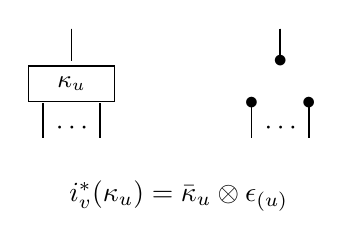
\begin{tikzpicture}[xscale = .5, yscale = .55, baseline=(current  bounding  box.center)]
\begin{pgfonlayer}{nodelayer}
		\node [style=none] (210) at (1.9, 4.3) {};
		\node [style=none] (211) at (1.9, 3.55) {};
		\node [style=wide small box] (225) at (1.9, 3.025) {$\kappa_u$};
		\node [style=none] (226) at (1.175, 2.575) {};
		\node [style=none] (227) at (1.175, 1.775) {};
		\node [style=none] (228) at (2.625, 2.575) {};
		\node [style=none] (229) at (2.625, 1.775) {};
		\node [style=none] (286) at (4.625, 2.925) {$\efun$};
		\node [style=none] (295) at (1.97, 2) {$\cdots$};
		\node [style=none] (296) at (7.2, 4.3) {};
		\node [style=none] (297) at (7.2, 3.55) {$\bullet$};
		\node [style=none] (299) at (6.475, 2.575) {$\bullet$};
		\node [style=none] (300) at (6.475, 1.775) {};
		\node [style=none] (301) at (7.925, 2.575) {$\bullet$};
		\node [style=none] (302) at (7.925, 1.775) {};
		\node [style=none] (304) at (7.27, 2) {$\cdots$};
		\node [style=none] (305) at (4.625, 0.425) {$i_{v}^*(\kappa_u) = \bar \kappa_u \otimes \epsilon_{\pa(u)}$};
	\end{pgfonlayer}
	\begin{pgfonlayer}{edgelayer}
		\draw [style=wire] (210.center) to (211.center);
		\draw [style=wire] (226.center) to (227.center);
		\draw [style=wire] (228.center) to (229.center);
		\draw [style=wire] (210.center) to (211.center);
		\draw [style=wire] (226.center) to (227.center);
		\draw [style=wire] (228.center) to (229.center);
		\draw [style=wire] (296.center) to (297.center);
		\draw [style=wire] (299.center) to (300.center);
		\draw [style=wire] (301.center) to (302.center);
		\draw [style=wire] (296.center) to (297.center);
		\draw [style=wire] (299.center) to (300.center);
		\draw [style=wire] (301.center) to (302.center);
	\end{pgfonlayer}
\end{tikzpicture}
\end{equation}
where $\kappa_u$, $\bar \kappa_u$ are the causal mechanisms on $u$ in $\cau(G)$, $\cau(G_{\bar v})$, respectively. Indeed, $i_v^{-1}(u) = u$ for every atomic variable $u$, so the discard and the duplicate on $u$ are sent to the discard and the duplicate on $u$. If $u \notin v$ then $u$ has the same parents in both graphs, and $[u \| \pa_G(u)]$ in $\cau(G_{\bar v})$ is the causal mechanism on $u$. If $u \in v$ then no directed path of $G_{\bar v}$ ends in $u$, so $[u \| \pa_G(u)]$ consists of $\bar \kappa_u$ and the discards on the parents of $u$ in $G$.

In the definition of $\cau(G)$, we do not have an exogenous causal mechanism $\0 \fun w$ for every $w \in V_G$ unless $w$ has no parents in $G$. Of course, such generators, indeed, arbitrary generators, can be introduced to suit the task at hand. In that case, there is no need to go through this subgraph $G_{\bar v}$ anymore. If an arrow $\bar \kappa_w : \0 \fun w$ is added to $W(G)$ for every $w \in V_G$ then (\ref{inter:exam}), together with the assignment that fixes the discards, the duplicates, the causal mechanisms $\kappa_u$ with $u \notin v$, and all the new arrows $\bar \kappa_w$, defines a strict Markov endofunctor of the free Markov category over the enlarged graph monoid, which takes the place of $i_{v}^*$. This is the approach adopted  in \cite{jacobs2019causal}, where a specific interpretation is intended for these exogenous causal mechanisms, namely uniform probability distribution. Casting $i_{v}^*$ as an endofunctor is merely for convenience and elegance, though, not a technical necessity.
\end{exam}




\begin{prop}\label{cond:preserve}
Let $v$, $w$ be singular variables in $\cau(G)$. Then $\phi^*([w \| v]) = [\phi^*(w) \| \phi^*(v)]$.
\end{prop}

This assertion is a bit terse  and may seem to be just a consequence of Proposition~\ref{mar:fun:eff}. But the situation   becomes clearer if we do not abbreviate the notation:
\begin{equation}\label{comp:two}
\bfig \morphism(0,0)/=/<1450,0>[[\phi^*(w) \| \phi^*(v)]_{( \phi^*(V_G), \phi^*(K_G))}`\phi^*([w \| v]_{(V_G, K_G)}); \textup{Proposition~\ref{mar:fun:eff}}]
\morphism(1450,0)/=/<1330,0>[\phantom{\phi^*([w \| v]_{(V_G, K_G)})}`[\phi^*(w) \| \phi^*(v)]_{(V_H, K_H)}; \textup{Proposition~\ref{cond:preserve}}]
\efig
\end{equation}
where $K_G$, $K_H$ are the families of Definition~\ref{cau:condi} for $G$, $H$, and $\phi^*(V_G)$, $\phi^*(K_G)$ are as in Proposition~\ref{mar:fun:eff}. So in the first effect the objects are the words $\phi^{-1}(y)$, $y \in V_G$, some of which may be empty, and the morphisms are the effects $\phi^*(\kappa_y)$ of (\ref{sub:fun:gen}), whereas in the last one the objects are the vertices of $H$ and the morphisms are its causal mechanisms.

\begin{proof}
We first reduce to the case that $v = v_S$ and $w = v_T$ for some $S, T \sub \{1, \ldots, n\}$. In general $[w \| v] = \tau_* \circ [v_T \| v_S] \circ \rho_*^{-1}$, as in Definition~\ref{cau:condi}. Since $\phi^*$ is a strict symmetric monoidal functor, $\phi^*(\tau_*)$ is represented by the diagram without nodes in which each atomic variable in $\phi^{-1}(v_T)$ is connected with the same atomic variable in $\phi^{-1}(w)$, and similarly for $\rho_*$. So, by Definition~\ref{cau:condi} for $H$, $[\phi^*(w) \| \phi^*(v)] = \phi^*(\tau_*) \circ [\phi^*(v_T) \| \phi^*(v_S)] \circ \phi^*(\rho_*)^{-1}$.

So let $v = v_S$ and $w = v_T$. We identify $S$, $T$ with the corresponding sets of vertices of $G$, and write $S' = \phi^{-1}(S)$, $T' = \phi^{-1}(T)$, $D = V(G_{S \rightarrow T})$, and $D' = V(H_{S' \rightarrow T'})$. Thus $\phi^*(v)$, $\phi^*(w)$ consist of the vertices in $S'$, $T'$, in the order of $V_H$. The letters $x$, $p$ stand for vertices of $H$ and the letter $y$ for vertices of $G$.

Let $\Gamma_G$ be a diagram $\stri_{[w \| v]_{(V_G, K_G)}}$ with the multipliers in binary form. By its construction in Definition~\ref{gen:condi}, it has exactly one node with the value $\kappa_y$ for each $y \in D \mi S$, whose inputs correspond to the parents of $y$, its other nodes are duplicates and discards, and
\begin{itemize}
  \item[($*$)] for every edge $e$ with the value $y$, the origin $e^{\circ}$ is the edge in the domain with the value $y$ if $y \in S$, and is the output of the node with the value $\kappa_y$ if $y \notin S$.
\end{itemize}
The same holds for the effect diagrams in $W(H)$. Let $\Gamma_H$ be a diagram of the last effect in (\ref{comp:two}), with the multipliers in binary form; its node with the value $\kappa_x$ is live for every $x \in D' \mi S'$, as noted in Definition~\ref{gen:condi}.

Let $\Gamma_{\phi^* G}$ be the diagram in $W(H)$ obtained from $\Gamma_G$ as follows. Every edge with the value $y$ is replaced by one edge for each atomic variable in $\phi^{-1}(y)$, in their order. Every duplicate or discard on $y$ is replaced by the duplicates or discards on the atomic variables in $\phi^{-1}(y)$, with the outputs of the duplicates arranged as $\phi^{-1}(y) \phi^{-1}(y)$. The node with the value $\kappa_y$ is replaced by a diagram $B_y$ of the effect $[\phi^{-1}(y) \| \phi^{-1}(\pa(y))]_{(V_H, K_H)}$ with the multipliers in binary form. These are diagrams of the images under $\phi^*$ of the values of the nodes of $\Gamma_G$, by (\ref{sub:fun:gen}), and $\phi^*$ is a strict symmetric monoidal functor; so $\Gamma_{\phi^* G}$ represents $\phi^*([w \| v])$, compare the proof of Proposition~\ref{mar:fun:eff}. By the note after (\ref{sub:fun:gen}), the nodes of $B_y$ are one node with the value $\kappa_x$ for each $x \in \phi^{-1}(y)$, duplicates, and discards. So, for each $x \in \phi^{-1}(D \mi S)$, there is exactly one node of $\Gamma_{\phi^* G}$ with the value $\kappa_x$, which we denote by $k_x$, and the other nodes of $\Gamma_{\phi^* G}$ are duplicates and discards.

We claim that ($*$) holds in $\Gamma_{\phi^* G}$ in the following form: for every edge $e$ with the value $p$, the origin $e^{\circ}$ is the edge in the domain with the value $p$ if $p \in S'$, and is the output of $k_p$ if $p \notin S'$. Suppose first that $e$ is one of the edges that replace an edge $e_0$ of $\Gamma_G$, with the value $y = \phi(p)$. Following $e$ backward through the duplicates on $p$, we arrive at the edge with the value $p$ among those that replace $e_0^{\circ}$. If $y \in S$ then, by ($*$) in $\Gamma_G$, this is the edge in the domain with the value $p$. If $y \notin S$ then it is the edge with the value $p$ in the codomain of $B_y$, whose origin is the output of $k_p$, by ($*$) in $B_y$. Suppose next that $e$ is an edge of some $B_y$. By ($*$) in $B_y$, its origin in $B_y$ is the output of $k_p$ if $p \in \phi^{-1}(y)$, and is otherwise the edge with the value $p$ in the domain of $B_y$, which is one of the edges that replace an input of the node with the value $\kappa_y$ in $\Gamma_G$; so we are back in the first case.

The inputs of $k_x$ correspond to the parents of $x$ in $H$. So the claim yields: the output of $k_p$ is the origin of an input of $k_x$ if and only if $p \notin S'$ and $p$ is a parent of $x$, and it is the origin of an edge in the codomain if and only if $p \in T' \mi S'$. Now we determine the live nodes of $\Gamma_{\phi^* G}$; they are among the nodes $k_x$, since the other nodes are duplicates and discards. If a directed path leads from $k_x$ to the codomain then the nodes on it that are not duplicates are $k_{p_0}, \ldots, k_{p_r}$ with $p_0 = x$, the output of $k_{p_i}$ is the origin of an input of $k_{p_{i+1}}$, and the output of $k_{p_r}$ is the origin of an edge in the codomain. So $p_0, \ldots, p_r$ form a directed path in $H$ that ends in $T'$ and does not contain any vertex in $S'$, and hence $x \in D' \mi S'$. Conversely, let $x \in D' \mi S'$. Then there is a directed path $p_0, \ldots, p_r$ in $H$ with $p_0 = x$ and $p_r \in T'$ that does not contain any vertex in $S'$ (if $x \in T'$ then $r = 0$). Erasing the repetitions in $\phi(p_0), \ldots, \phi(p_r)$ gives a directed path in $G$ that ends in $T$ and does not contain any vertex in $S$; so $\phi(p_i) \in D \mi S$ and the node $k_{p_i}$ exists for every $i$. By the claim, a directed path leads from $k_{p_i}$ to $k_{p_{i+1}}$ and from $k_{p_r}$ to the codomain. So $k_x$ is live.

Therefore the live nodes of $\Gamma_{\phi^* G}$ are the nodes $k_x$, $x \in D' \mi S'$, and so are those of $\Gamma_H$, with the same values. By the claim and by ($*$) in $\Gamma_H$, in both diagrams the origin of an edge in the codomain, or of an input of a live node, with the value $p$ is the edge in the domain with the value $p$ if $p \in S'$, and is the output of the live node with the value $\kappa_p$ otherwise. So $\Gamma_{\phi^* G}$ and $\Gamma_H$ have the same skeleton, and hence represent the same morphism, by Lemma~\ref{mar:min:com}.
\end{proof}

%
%



\begin{thm}[Functoriality of refinement]\label{int:func}
The construction of $\phi^*$ is functorial, that is, there is a contravariant  functor
\[
\intv : \cat{FinODAG} \fun \cat{MarCat}
\]
sending each object  $G \in  \cat{FinODAG}$ to $\cau(G)$ and each morphism $\phi \in  \cat{FinODAG}$ to $\phi^*$.
\end{thm}
\begin{proof}
Since $\phi^*$ is a Markov functor $\cau(G) \fun \cau(H)$ for every morphism $\phi : H \fun G$, we need to check that identities and compositions are respected.

Let $\phi$ be the identity on $G$. Then $\phi^{-1}(v) = v$ for every variable $v$ and, for every atomic variable $v$, $f_\phi(\kappa_v) = [v \| \pa(v)] = \kappa_v$: by Definition~\ref{gen:condi}, the diagram of this effect consists of the node with the value $\kappa_v$, since every parent of $v$ has exactly one child in $G_{\pa(v) \rightarrow v}$. So $f_\phi$ is the graph monoid homomorphism $W(G) \fun \cau(G)$ that comes with the free Markov category, and hence $\phi^*$ is the identity functor, by the uniqueness in Definition~\ref{phi:inter}.

Let $G'' \to^\psi G' \to^\phi G$ be morphisms in $\cat{FinODAG}$. We show that $\psi^* \circ \phi^* = (\phi \circ \psi)^*$. Both are strict Markov functors $\cau(G) \fun \cau(G'')$. So, by the uniqueness in Definition~\ref{phi:inter}, it is enough to check that $\psi^* \circ \phi^*$ agrees with $f_{\phi \circ \psi}$ on $W(G)$. For an atomic variable $v$, the words $\psi^{-1}(\phi^{-1}(v))$ and $(\phi \circ \psi)^{-1}(v)$ have the same atomic variables, and the first one lists them block by block, a block being a fiber of $\psi$ over a vertex in $\phi^{-1}(v)$; since the fibers of $\psi$ are ordered as their images, this is the order of $V_{G''}$, and so the two words are equal. Hence $\psi^{-1}(\phi^{-1}(v)) = (\phi \circ \psi)^{-1}(v)$ for all variables $v$. Since a strict Markov functor matches the duplicates and the discards on all objects,
\[
\psi^*(\phi^*(\epsilon_v)) = \psi^*(\epsilon_{\phi^{-1}(v)}) = \epsilon_{\psi^{-1}(\phi^{-1}(v))} = f_{\phi \circ \psi}(\epsilon_v),
\]
and similarly for $\delta_v$. Finally, by Proposition~\ref{cond:preserve}, applied to $\psi$ and the singular variables $\phi^{-1}(v)$, $\phi^{-1}(\pa(v))$ in $\cau(G')$,
\[
\psi^*(\phi^*(\kappa_v)) = \psi^*([\phi^{-1}(v) \| \phi^{-1}(\pa(v))]) = [\psi^{-1}(\phi^{-1}(v)) \| \psi^{-1}(\phi^{-1}(\pa(v)))] = f_{\phi \circ \psi}(\kappa_v). \qedhere
\]
\end{proof}


\providecommand{\bysame}{\leavevmode\hbox to3em{\hrulefill}\thinspace}
\providecommand{\MR}{\relax\ifhmode\unskip\space\fi MR }
% \MRhref is called by the amsart/book/proc definition of \MR.
\providecommand{\MRhref}[2]{%
  \href{http://www.ams.org/mathscinet-getitem?mr=#1}{#2}
}
\providecommand{\href}[2]{#2}
\begin{thebibliography}{1}

\bibitem{Fong:thesis}
Brendan Fong, \emph{Causal theories: {A} categorical perspective on {B}ayesian
  networks},  (2013), arXiv:1301.6201.

\bibitem{fritz2020synthetic}
Tobias Fritz, \emph{A synthetic approach to {M}arkov kernels, conditional
  independence and theorems on sufficient statistics}, Advances in Mathematics
  \textbf{370} (2020), 107239.

\bibitem{FriLiang2022}
Tobias Fritz and Wendong Liang, \emph{Free gs-monoidal categories and free
  {M}arkov categories}, Applied Categorical Structures \textbf{31} (2023),
  article~21, arXiv:2204.02284.

\bibitem{jacobs2019causal}
Bart Jacobs, Aleks Kissinger, and Fabio Zanasi, \emph{Causal inference by
  string diagram surgery}, International conference on foundations of software
  science and computation structures, Springer, 2019, pp.~313--329.

\bibitem{joyal1991geometry}
Andr{\'e} Joyal and Ross Street, \emph{The geometry of tensor calculus, {I}},
  Advances in mathematics \textbf{88} (1991), no.~1, 55--112.

\bibitem{maclane1985coherence}
Saunders MacLane and Robert Par{\'e}, \emph{Coherence for bicategories and
  indexed categories}, Journal of Pure and Applied Algebra \textbf{37} (1985),
  59--80.

\bibitem{selinger2010survey}
Peter Selinger, \emph{A survey of graphical languages for monoidal categories},
  New structures for physics, Springer, 2010, pp.~289--355.

\bibitem{yinzhang2021}
Yimu Yin and Jiji Zhang, \emph{{M}arkov categories, causal theories, and the
  do-calculus}, Studies in Logic \textbf{14} (2021), 1--24.

\end{thebibliography}



\end{document}




